% Options for packages loaded elsewhere
\PassOptionsToPackage{unicode}{hyperref}
\PassOptionsToPackage{hyphens}{url}
\PassOptionsToPackage{dvipsnames,svgnames,x11names}{xcolor}
\PassOptionsToPackage{space}{xeCJK}
%
\documentclass[
  a4paper,
  fontset=none,
]{ctexart}
\usepackage{amsmath,amssymb}
\usepackage{iftex}
\ifPDFTeX
  \usepackage[T1]{fontenc}
  \usepackage[utf8]{inputenc}
  \usepackage{textcomp} % provide euro and other symbols
\else % if luatex or xetex
  \usepackage{unicode-math} % this also loads fontspec
  \defaultfontfeatures{Scale=MatchLowercase}
  \defaultfontfeatures[\rmfamily]{Ligatures=TeX,Scale=1}
\fi
\usepackage{lmodern}
\ifPDFTeX\else
  % xetex/luatex font selection
  \setmainfont[]{Noto Serif}
  \setmonofont[]{Noto Sans Mono}
  \ifXeTeX
    \usepackage{xeCJK}
    \setCJKmainfont[AutoFakeSlant=0.15]{Noto Sans CJK SC}
    \setCJKmonofont[AutoFakeSlant=0.15]{Noto Sans CJK SC}
          \fi
  \ifLuaTeX
    \usepackage[]{luatexja-fontspec}
    \setmainjfont[]{Noto Sans CJK SC}
  \fi
\fi
% Use upquote if available, for straight quotes in verbatim environments
\IfFileExists{upquote.sty}{\usepackage{upquote}}{}
\IfFileExists{microtype.sty}{% use microtype if available
  \usepackage[]{microtype}
  \UseMicrotypeSet[protrusion]{basicmath} % disable protrusion for tt fonts
}{}
\makeatletter
\@ifundefined{KOMAClassName}{% if non-KOMA class
  \IfFileExists{parskip.sty}{%
    \usepackage{parskip}
  }{% else
    \setlength{\parindent}{0pt}
    \setlength{\parskip}{6pt plus 2pt minus 1pt}}
}{% if KOMA class
  \KOMAoptions{parskip=half}}
\makeatother
\usepackage{xcolor}
\usepackage[margin=2.3cm]{geometry}
\usepackage{color}
\usepackage{fancyvrb}
\newcommand{\VerbBar}{|}
\newcommand{\VERB}{\Verb[commandchars=\\\{\}]}
\DefineVerbatimEnvironment{Highlighting}{Verbatim}{commandchars=\\\{\}}
% Add ',fontsize=\small' for more characters per line
\newenvironment{Shaded}{}{}
\newcommand{\AlertTok}[1]{\textcolor[rgb]{1.00,0.00,0.00}{\textbf{#1}}}
\newcommand{\AnnotationTok}[1]{\textcolor[rgb]{0.38,0.63,0.69}{\textbf{\textit{#1}}}}
\newcommand{\AttributeTok}[1]{\textcolor[rgb]{0.49,0.56,0.16}{#1}}
\newcommand{\BaseNTok}[1]{\textcolor[rgb]{0.25,0.63,0.44}{#1}}
\newcommand{\BuiltInTok}[1]{\textcolor[rgb]{0.00,0.50,0.00}{#1}}
\newcommand{\CharTok}[1]{\textcolor[rgb]{0.25,0.44,0.63}{#1}}
\newcommand{\CommentTok}[1]{\textcolor[rgb]{0.38,0.63,0.69}{\textit{#1}}}
\newcommand{\CommentVarTok}[1]{\textcolor[rgb]{0.38,0.63,0.69}{\textbf{\textit{#1}}}}
\newcommand{\ConstantTok}[1]{\textcolor[rgb]{0.53,0.00,0.00}{#1}}
\newcommand{\ControlFlowTok}[1]{\textcolor[rgb]{0.00,0.44,0.13}{\textbf{#1}}}
\newcommand{\DataTypeTok}[1]{\textcolor[rgb]{0.56,0.13,0.00}{#1}}
\newcommand{\DecValTok}[1]{\textcolor[rgb]{0.25,0.63,0.44}{#1}}
\newcommand{\DocumentationTok}[1]{\textcolor[rgb]{0.73,0.13,0.13}{\textit{#1}}}
\newcommand{\ErrorTok}[1]{\textcolor[rgb]{1.00,0.00,0.00}{\textbf{#1}}}
\newcommand{\ExtensionTok}[1]{#1}
\newcommand{\FloatTok}[1]{\textcolor[rgb]{0.25,0.63,0.44}{#1}}
\newcommand{\FunctionTok}[1]{\textcolor[rgb]{0.02,0.16,0.49}{#1}}
\newcommand{\ImportTok}[1]{\textcolor[rgb]{0.00,0.50,0.00}{\textbf{#1}}}
\newcommand{\InformationTok}[1]{\textcolor[rgb]{0.38,0.63,0.69}{\textbf{\textit{#1}}}}
\newcommand{\KeywordTok}[1]{\textcolor[rgb]{0.00,0.44,0.13}{\textbf{#1}}}
\newcommand{\NormalTok}[1]{#1}
\newcommand{\OperatorTok}[1]{\textcolor[rgb]{0.40,0.40,0.40}{#1}}
\newcommand{\OtherTok}[1]{\textcolor[rgb]{0.00,0.44,0.13}{#1}}
\newcommand{\PreprocessorTok}[1]{\textcolor[rgb]{0.74,0.48,0.00}{#1}}
\newcommand{\RegionMarkerTok}[1]{#1}
\newcommand{\SpecialCharTok}[1]{\textcolor[rgb]{0.25,0.44,0.63}{#1}}
\newcommand{\SpecialStringTok}[1]{\textcolor[rgb]{0.73,0.40,0.53}{#1}}
\newcommand{\StringTok}[1]{\textcolor[rgb]{0.25,0.44,0.63}{#1}}
\newcommand{\VariableTok}[1]{\textcolor[rgb]{0.10,0.09,0.49}{#1}}
\newcommand{\VerbatimStringTok}[1]{\textcolor[rgb]{0.25,0.44,0.63}{#1}}
\newcommand{\WarningTok}[1]{\textcolor[rgb]{0.38,0.63,0.69}{\textbf{\textit{#1}}}}
\usepackage{longtable,booktabs,array}
\usepackage{calc} % for calculating minipage widths
% Correct order of tables after \paragraph or \subparagraph
\usepackage{etoolbox}
\makeatletter
\patchcmd\longtable{\par}{\if@noskipsec\mbox{}\fi\par}{}{}
\makeatother
% Allow footnotes in longtable head/foot
\IfFileExists{footnotehyper.sty}{\usepackage{footnotehyper}}{\usepackage{footnote}}
\makesavenoteenv{longtable}
\usepackage{graphicx}
\makeatletter
\def\maxwidth{\ifdim\Gin@nat@width>\linewidth\linewidth\else\Gin@nat@width\fi}
\def\maxheight{\ifdim\Gin@nat@height>.86\textheight .86\textheight\else\Gin@nat@height\fi}
\makeatother
% Scale images if necessary, so that they will not overflow the page
% margins by default, and it is still possible to overwrite the defaults
% using explicit options in \includegraphics[width, height, ...]{}
\setkeys{Gin}{width=\maxwidth,height=\maxheight,keepaspectratio}
% Set default figure placement to htbp
\makeatletter
\def\fps@figure{htbp}
\makeatother
\graphicspath{{./}{../}}
\setlength{\emergencystretch}{6em} % prevent overfull lines
\sloppy
\providecommand{\tightlist}{%
  \setlength{\itemsep}{0pt}\setlength{\parskip}{0pt}}
\setcounter{secnumdepth}{-\maxdimen} % remove section numbering
\ifLuaTeX
  \usepackage{selnolig}  % disable illegal ligatures
\fi
\IfFileExists{bookmark.sty}{\usepackage{bookmark}}{\usepackage{hyperref}}
\IfFileExists{xurl.sty}{\usepackage{xurl}}{} % add URL line breaks if available
\urlstyle{same}
\hypersetup{
  colorlinks=true,
  linkcolor={black},
  filecolor={Maroon},
  citecolor={Blue},
  urlcolor={blue},
  pdfcreator={LaTeX via pandoc}}

\title{编译原理实验报告}
\author{郑天白（23070202）\and 段晰迈（23070201）\and 高子涵（23070207）}
\date{}

\begin{document}

\maketitle
\tableofcontents
\newpage

\hypertarget{ux5b9eux9a8cux57faux672cux4fe1ux606f}{%
\subsection{1.
实验基本信息}\label{ux5b9eux9a8cux57faux672cux4fe1ux606f}}

\begin{longtable}[]{@{}ll@{}}
\toprule\noalign{}
项目 & 内容 \\
\midrule\noalign{}
\endhead
\bottomrule\noalign{}
\endlastfoot
课程 & 编译原理 \\
实验一 & 词法分析程序的设计与实现 \\
实验二/三 & 语法制导的三地址代码生成 \\
实现语言 & Java \\
自动生成工具 & GNU Bison，Java parser 输出 \\
可执行程序 & \texttt{dist/compiler-lab.jar} \\
构建命令 & \texttt{make\ build}、\texttt{make\ dist} \\
测试命令 & \texttt{make\ test} \\
验证结果 & 2026-05-29 执行 \texttt{date\ \&\&\ make\ test} 通过 \\
\end{longtable}

\hypertarget{ux5b9eux9a8cux4efbux52a1ux5206ux5de5}{%
\subsection{2.
实验任务分工}\label{ux5b9eux9a8cux4efbux52a1ux5206ux5de5}}

本组按照实验任务划分，亦即编译器前端处理流程分工。三位成员均参与总体设计与联调，具体分工如下。

\begin{longtable}[]{@{}
  >{\raggedright\arraybackslash}p{(\columnwidth - 6\tabcolsep) * \real{0.2500}}
  >{\raggedright\arraybackslash}p{(\columnwidth - 6\tabcolsep) * \real{0.2500}}
  >{\raggedright\arraybackslash}p{(\columnwidth - 6\tabcolsep) * \real{0.2500}}
  >{\raggedright\arraybackslash}p{(\columnwidth - 6\tabcolsep) * \real{0.2500}}@{}}
\toprule\noalign{}
\begin{minipage}[b]{\linewidth}\raggedright
成员
\end{minipage} & \begin{minipage}[b]{\linewidth}\raggedright
学号
\end{minipage} & \begin{minipage}[b]{\linewidth}\raggedright
主要分工
\end{minipage} & \begin{minipage}[b]{\linewidth}\raggedright
主要技术内容
\end{minipage} \\
\midrule\noalign{}
\endhead
\bottomrule\noalign{}
\endlastfoot
郑天白 & 23070202 & 词法分析子系统 & 输入处理、Token
识别、正规式、正规文法、状态图、词法测试 \\
段晰迈 & 23070201 & 递归下降语法分析子系统 &
消除左递归、递归下降子程序、语法图、语法树输出、错误处理扩展 \\
高子涵 & 23070207 & Bison 语法分析与三地址代码生成 & Bison
文法、MiniYacc/SLR demo 程序、AST、TAC
生成、错误恢复、扩展功能、测试、可执行程序 \\
\end{longtable}

报告按编译器前端流程统一组织，将词法分析、递归下降语法分析、Bison
语法分析、MiniYacc/SLR
原理展示和三地址代码生成放入同一条技术主线中说明。

\hypertarget{ux5b9eux9a8cux8981ux6c42ux5b8cux6210ux60c5ux51b5}{%
\subsection{3.
实验要求完成情况}\label{ux5b9eux9a8cux8981ux6c42ux5b8cux6210ux60c5ux51b5}}

\begin{longtable}[]{@{}
  >{\raggedright\arraybackslash}p{(\columnwidth - 4\tabcolsep) * \real{0.3800}}
  >{\raggedright\arraybackslash}p{(\columnwidth - 4\tabcolsep) * \real{0.1200}}
  >{\raggedright\arraybackslash}p{(\columnwidth - 4\tabcolsep) * \real{0.5000}}@{}}
\toprule\noalign{}
\begin{minipage}[b]{\linewidth}\raggedright
实验要求
\end{minipage} & \begin{minipage}[b]{\linewidth}\raggedright
完成情况
\end{minipage} & \begin{minipage}[b]{\linewidth}\raggedright
证据
\end{minipage} \\
\midrule\noalign{}
\endhead
\bottomrule\noalign{}
\endlastfoot
词法分析器识别三种整数、标识符、主要运算符和关键字 & 已完成 &
\texttt{examples/lab1/handout.*}、\texttt{tests/lab1\_sample.*} \\
给出词法正规式、正规文法、状态图、主要数据结构与算法 & 已完成 & 本报告第
4 节 \\
语法分析程序输出语法树或最左派生产生式序列 & 已完成 &
\texttt{examples/lab2/tree-sample.*}、\texttt{tests/lab2\_tree\_sample.*} \\
源程序包含多个语句 & 已完成 & 标准 Lab 2/Lab 3 样例均包含多语句 \\
对源程序错误做适当处理 & 已完成 &
\texttt{tests/lab2\_tree\_invalid\_octal.*}、\texttt{tests/lab3\_tac\_error\_*} \\
根据语法制导定义生成三地址代码 & 已完成 &
\texttt{examples/lab3/handout-tac.*}、\texttt{tests/lab3\_tac\_sample.*} \\
采用自动生成技术时说明工具、描述程序和辅助程序 & 已完成 & 第 5.2 节
Bison 语法分析 \\
扩展功能 & 已完成 & 关系运算、复合语句、错误恢复、AST
展示、常量折叠、MiniYacc/SLR 展示 \\
可执行程序 & 已完成 & \texttt{make\ dist} 生成
\texttt{dist/compiler-lab.jar} \\
\end{longtable}

\hypertarget{ux8bcdux6cd5ux5206ux6790ux5b50ux7cfbux7edf}{%
\subsection{4.
词法分析子系统}\label{ux8bcdux6cd5ux5206ux6790ux5b50ux7cfbux7edf}}

\hypertarget{ux5b50ux7cfbux7edfux4efbux52a1}{%
\subsubsection{4.1 子系统任务}\label{ux5b50ux7cfbux7edfux4efbux52a1}}

词法分析子系统负责从标准输入读取源程序，将字符序列转换为具有种别值和属性值的
Token。实验要求识别：

\begin{enumerate}
\def\labelenumi{\arabic{enumi}.}
\tightlist
\item
  标识符；
\item
  十进制整数；
\item
  八进制整数；
\item
  十六进制整数；
\item
  主要运算符和分隔符；
\item
  关键字；
\item
  非法八进制整数；
\item
  非法十六进制整数。
\end{enumerate}

本组词法分析程序采用手工实现方式，没有使用
Lex/Flex。程序先读取完整标准输入，再逐个扫描
token。\texttt{src/Lexer.java} 与 \texttt{src/Token.java} 是 Lab 1、Lab
2、Lab 3 共用的词法实现。

\hypertarget{ux5b57ux7b26ux96c6ux4e0eux6b63ux89c4ux5f0f}{%
\subsubsection{4.2
字符集与正规式}\label{ux5b57ux7b26ux96c6ux4e0eux6b63ux89c4ux5f0f}}

字符集定义：

\begin{Shaded}
\begin{Highlighting}[]
\NormalTok{letter             = A|B|...|Z|a|b|...|z}
\NormalTok{digit              = 0|1|2|3|4|5|6|7|8|9}
\NormalTok{nonzero\_digit      = 1|2|3|4|5|6|7|8|9}
\NormalTok{oct\_digit          = 0|1|2|3|4|5|6|7}
\NormalTok{hex\_digit          = digit|a|b|c|d|e|f|A|B|C|D|E|F}
\NormalTok{illegal\_hex\_letter = g|h|...|z|G|H|...|Z}
\NormalTok{underline          = \_}
\NormalTok{id\_start           = letter|underline}
\NormalTok{id\_char            = letter|digit|underline}
\end{Highlighting}
\end{Shaded}

指导书中标识符正规式为：

\begin{Shaded}
\begin{Highlighting}[]
\NormalTok{IDN = letter(letter|digit)*}
\end{Highlighting}
\end{Shaded}

实现中扩展支持下划线，因此实际标识符正规式为：

\begin{Shaded}
\begin{Highlighting}[]
\NormalTok{IDN = (letter|\_)(letter|digit|\_)*}
\end{Highlighting}
\end{Shaded}

整数正规式：

\begin{Shaded}
\begin{Highlighting}[]
\NormalTok{DEC   = 0 | nonzero\_digit digit*}
\NormalTok{OCT   = 0 oct\_digit+}
\NormalTok{HEX   = 0(x|X)hex\_digit+}
\NormalTok{ILOCT = 0 digit* (8|9) digit*}
\NormalTok{ILHEX = 0(x|X)(digit|letter)* illegal\_hex\_letter (digit|letter)*}
\end{Highlighting}
\end{Shaded}

关键字正规式：

\begin{Shaded}
\begin{Highlighting}[]
\NormalTok{KEYWORD = if|then|else|while|do|begin|end}
\end{Highlighting}
\end{Shaded}

运算符和分隔符正规式：

\begin{Shaded}
\begin{Highlighting}[]
\NormalTok{OP        = +|{-}|*|/|\textgreater{}|\textless{}|=|\textgreater{}=|\textless{}=|\textless{}\textgreater{}}
\NormalTok{DELIMITER = (|)|;}
\end{Highlighting}
\end{Shaded}

\hypertarget{ux5355ux8bcdux79cdux522bux8bbeux7f6e}{%
\subsubsection{4.3
单词种别设置}\label{ux5355ux8bcdux79cdux522bux8bbeux7f6e}}

\begin{longtable}[]{@{}lll@{}}
\toprule\noalign{}
单词 & 种别值 & 属性值 \\
\midrule\noalign{}
\endhead
\bottomrule\noalign{}
\endlastfoot
标识符 & \texttt{IDN} & 字符串 \\
十进制整数 & \texttt{DEC} & 数值 \\
八进制整数 & \texttt{OCT} & 数值 \\
十六进制整数 & \texttt{HEX} & 数值 \\
\texttt{+} & \texttt{ADD} & \texttt{-} \\
\texttt{-} & \texttt{SUB} & \texttt{-} \\
\texttt{*} & \texttt{MUL} & \texttt{-} \\
\texttt{/} & \texttt{DIV} & \texttt{-} \\
\texttt{\textgreater{}} & \texttt{GT} & \texttt{-} \\
\texttt{\textless{}} & \texttt{LT} & \texttt{-} \\
\texttt{=} & \texttt{EQ} & \texttt{-} \\
\texttt{\textgreater{}=} & \texttt{GE} & \texttt{-} \\
\texttt{\textless{}=} & \texttt{LE} & \texttt{-} \\
\texttt{\textless{}\textgreater{}} & \texttt{NEQ} & \texttt{-} \\
\texttt{(} & \texttt{SLP} & \texttt{-} \\
\texttt{)} & \texttt{SRP} & \texttt{-} \\
\texttt{;} & \texttt{SEMI} & \texttt{-} \\
\texttt{if} & \texttt{IF} & \texttt{-} \\
\texttt{then} & \texttt{THEN} & \texttt{-} \\
\texttt{else} & \texttt{ELSE} & \texttt{-} \\
\texttt{while} & \texttt{WHILE} & \texttt{-} \\
\texttt{do} & \texttt{DO} & \texttt{-} \\
\texttt{begin} & \texttt{BEGIN} & \texttt{-} \\
\texttt{end} & \texttt{END} & \texttt{-} \\
非法八进制数 & \texttt{ILOCT} & \texttt{-} \\
非法十六进制数 & \texttt{ILHEX} & \texttt{-} \\
其他非法数字 & \texttt{ILNUM} & \texttt{-} \\
无法识别词素 & \texttt{UNKNOWN} & 原词素 \\
\end{longtable}

\hypertarget{ux53d8ux6362ux540eux7684ux6b63ux89c4ux6587ux6cd5}{%
\subsubsection{4.4
变换后的正规文法}\label{ux53d8ux6362ux540eux7684ux6b63ux89c4ux6587ux6cd5}}

标识符和关键字：

\begin{Shaded}
\begin{Highlighting}[]
\NormalTok{S {-}\textgreater{} letter A | \_ A}
\NormalTok{A {-}\textgreater{} letter A | digit A | \_ A | ε}
\end{Highlighting}
\end{Shaded}

识别到字符串后再判断是否属于关键字表。如果属于
\texttt{if}、\texttt{then}、\texttt{else}、\texttt{while}、\texttt{do}、\texttt{begin}、\texttt{end}，则输出关键字种别；否则输出
\texttt{IDN}。

十进制整数：

\begin{Shaded}
\begin{Highlighting}[]
\NormalTok{S {-}\textgreater{} 0 | nonzero\_digit B}
\NormalTok{B {-}\textgreater{} digit B | ε}
\end{Highlighting}
\end{Shaded}

八进制整数：

\begin{Shaded}
\begin{Highlighting}[]
\NormalTok{S {-}\textgreater{} 0 C}
\NormalTok{C {-}\textgreater{} oct\_digit D}
\NormalTok{D {-}\textgreater{} oct\_digit D | ε}
\end{Highlighting}
\end{Shaded}

非法八进制整数：

\begin{Shaded}
\begin{Highlighting}[]
\NormalTok{S {-}\textgreater{} 0 E}
\NormalTok{E {-}\textgreater{} oct\_digit E | 8 F | 9 F}
\NormalTok{F {-}\textgreater{} digit F | ε}
\end{Highlighting}
\end{Shaded}

十六进制整数：

\begin{Shaded}
\begin{Highlighting}[]
\NormalTok{S {-}\textgreater{} 0 H}
\NormalTok{H {-}\textgreater{} x I | X I}
\NormalTok{I {-}\textgreater{} hex\_digit J}
\NormalTok{J {-}\textgreater{} hex\_digit J | ε}
\end{Highlighting}
\end{Shaded}

非法十六进制整数：

\begin{Shaded}
\begin{Highlighting}[]
\NormalTok{S {-}\textgreater{} 0 H}
\NormalTok{H {-}\textgreater{} x K | X K}
\NormalTok{K {-}\textgreater{} hex\_digit K | illegal\_hex\_letter L | ε}
\NormalTok{L {-}\textgreater{} digit L | letter L | ε}
\end{Highlighting}
\end{Shaded}

其中 \texttt{K\ -\textgreater{}\ ε} 覆盖 \texttt{0x} 或 \texttt{0X}
后没有任何十六进制数字的非法情况。

运算符和分隔符：

\begin{Shaded}
\begin{Highlighting}[]
\NormalTok{S {-}\textgreater{} + | {-} | * | / | = | ( | ) | ;}
\NormalTok{S {-}\textgreater{} \textgreater{} M}
\NormalTok{M {-}\textgreater{} = | ε}
\NormalTok{S {-}\textgreater{} \textless{} N}
\NormalTok{N {-}\textgreater{} = | \textgreater{} | ε}
\end{Highlighting}
\end{Shaded}

\hypertarget{ux72b6ux6001ux56fe}{%
\subsubsection{4.5 状态图}\label{ux72b6ux6001ux56fe}}

词法分析状态图如下。

\begin{figure}
\centering

\includegraphics{member-sources/lab1-media/media/image4.png}
\caption{Lab 1 词法分析状态图}
\end{figure}

从代码实现角度看，\texttt{Lexer.nextToken()} 的状态转换可以概括为：

\begin{Shaded}
\begin{Highlighting}[]
\NormalTok{start}
\NormalTok{  {-}\textgreater{} skipWhitespace}
\NormalTok{  {-}\textgreater{} relational operator branch}
\NormalTok{  {-}\textgreater{} single{-}character token branch}
\NormalTok{  {-}\textgreater{} collect lexeme}
\NormalTok{  {-}\textgreater{} keyword / identifier / number / unknown classification}
\end{Highlighting}
\end{Shaded}

\hypertarget{ux4e3bux8981ux6570ux636eux7ed3ux6784ux4e0eux51fdux6570}{%
\subsubsection{4.6
主要数据结构与函数}\label{ux4e3bux8981ux6570ux636eux7ed3ux6784ux4e0eux51fdux6570}}

\texttt{Token} 是词法分析输出的基本单位：

\begin{Shaded}
\begin{Highlighting}[]
\NormalTok{type   : token 种别值，如 IDN、DEC、WHILE}
\NormalTok{value  : 语义属性值，如标识符名、整数十进制值}
\NormalTok{lexeme : 原始词素，用于错误信息和非法 token 展示}
\NormalTok{line   : token 起始行}
\NormalTok{column : token 起始列}
\end{Highlighting}
\end{Shaded}

\texttt{Lexer} 保存输入状态：

\begin{Shaded}
\begin{Highlighting}[]
\NormalTok{input  : 完整输入字符串}
\NormalTok{pos    : 当前扫描位置}
\NormalTok{length : 输入长度}
\NormalTok{line   : 当前行号}
\NormalTok{column : 当前列号}
\end{Highlighting}
\end{Shaded}

关键函数：

\begin{longtable}[]{@{}
  >{\raggedright\arraybackslash}p{(\columnwidth - 2\tabcolsep) * \real{0.5000}}
  >{\raggedright\arraybackslash}p{(\columnwidth - 2\tabcolsep) * \real{0.5000}}@{}}
\toprule\noalign{}
\begin{minipage}[b]{\linewidth}\raggedright
函数
\end{minipage} & \begin{minipage}[b]{\linewidth}\raggedright
作用
\end{minipage} \\
\midrule\noalign{}
\endhead
\bottomrule\noalign{}
\endlastfoot
\texttt{Lexer.nextToken()} & 词法分析主函数，每次返回一个 token \\
\texttt{skipWhitespace()} & 跳过空格、制表符、换行符 \\
\texttt{singleCharacterToken()} & 识别单字符运算符和分隔符 \\
\texttt{classifyLexeme()} &
将完整词素分类为关键字、标识符、数字或未知 \\
\texttt{classifyNumber()} & 区分
\texttt{DEC}、\texttt{OCT}、\texttt{HEX}、\texttt{ILOCT}、\texttt{ILHEX}、\texttt{ILNUM} \\
\texttt{convertBaseToDecimal()} &
将八进制/十六进制属性值转换为十进制字符串 \\
\texttt{advancePos()} & 推进位置并维护行列号 \\
\end{longtable}

\hypertarget{ux8bcdux6cd5ux5206ux6790ux7b97ux6cd5}{%
\subsubsection{4.7
词法分析算法}\label{ux8bcdux6cd5ux5206ux6790ux7b97ux6cd5}}

\texttt{Lexer.nextToken()} 的算法流程：

\begin{Shaded}
\begin{Highlighting}[]
\NormalTok{1. 调用 skipWhitespace() 跳过空白符。}
\NormalTok{2. 如果输入结束，返回 null。}
\NormalTok{3. 记录当前 token 起始行列号。}
\NormalTok{4. 若当前字符为 \textgreater{}：}
\NormalTok{     若下一个字符为 =，返回 GE；}
\NormalTok{     否则返回 GT。}
\NormalTok{5. 若当前字符为 \textless{}：}
\NormalTok{     若下一个字符为 =，返回 LE；}
\NormalTok{     若下一个字符为 \textgreater{}，返回 NEQ；}
\NormalTok{     否则返回 LT。}
\NormalTok{6. 尝试识别单字符运算符和分隔符。}
\NormalTok{7. 向后读取直到空白符或运算符/分隔符，得到完整词素 lexeme。}
\NormalTok{8. classifyLexeme(lexeme)：}
\NormalTok{     先查关键字表；}
\NormalTok{     再判断标识符；}
\NormalTok{     再判断数字；}
\NormalTok{     否则返回 UNKNOWN。}
\NormalTok{9. classifyNumber(lexeme)：}
\NormalTok{     识别 0、十进制、八进制、十六进制；}
\NormalTok{     检测非法八进制、非法十六进制和其他非法数字。}
\end{Highlighting}
\end{Shaded}

八进制和十六进制的属性值通过 \texttt{convertBaseToDecimal(text,\ base)}
转为十进制字符串，便于语法分析和三地址代码生成直接使用。

\hypertarget{ux8bcdux6cd5ux5206ux6790ux6d4bux8bd5}{%
\subsubsection{4.8
词法分析测试}\label{ux8bcdux6cd5ux5206ux6790ux6d4bux8bd5}}

Lab 1
测试包含指导书样例运行验证，以及输入缓冲区行为验证。指导书样例运行结果如下。

\begin{figure}
\centering

\includegraphics{member-sources/lab1-media/media/image1.png}
\caption{Lab 1 指导书样例运行截图}
\end{figure}

输入缓冲区验证说明：编译器不会在用户每输入一个字符时立即分析，而是在完整输入交给程序后统一进行词法分析。组员通过修改
\texttt{0x1f} 输入验证该行为：在提交输入前将 \texttt{0x} 和 \texttt{1f}
中间加入空格，程序按最终输入分别识别；提交输入后再修改原输入不会改变已经进入分析流程的内容。

\begin{figure}
\centering

\includegraphics{member-sources/lab1-media/media/image2.png}
\caption{Lab 1 输入缓冲区提交前修改验证}
\end{figure}

\begin{figure}
\centering

\includegraphics{member-sources/lab1-media/media/image3.png}
\caption{Lab 1 输入缓冲区提交后修改验证}
\end{figure}

整合阶段补充的文本化样例用于自动化回归测试。运行命令：

\begin{Shaded}
\begin{Highlighting}[]
\ExtensionTok{java} \AttributeTok{{-}jar}\NormalTok{ dist/compiler{-}lab.jar lab1 }\OperatorTok{\textless{}}\NormalTok{ examples/lab1/handout.in}
\end{Highlighting}
\end{Shaded}

输入：

\begin{Shaded}
\begin{Highlighting}[]
\NormalTok{0 92+data\textgreater{}= 0x1f   09   ;}
\NormalTok{   while}
\end{Highlighting}
\end{Shaded}

输出：

\begin{Shaded}
\begin{Highlighting}[]
\NormalTok{DEC 0}
\NormalTok{DEC 92}
\NormalTok{ADD {-}}
\NormalTok{IDN data}
\NormalTok{GE {-}}
\NormalTok{HEX 31}
\NormalTok{ILOCT {-}}
\NormalTok{SEMI {-}}
\NormalTok{WHILE {-}}
\end{Highlighting}
\end{Shaded}

\hypertarget{ux8bedux6cd5ux5206ux6790ux5b50ux7cfbux7edf}{%
\subsection{5.
语法分析子系统}\label{ux8bedux6cd5ux5206ux6790ux5b50ux7cfbux7edf}}

语法分析子系统包括三部分：递归下降分析、Bison
自动生成语法分析器、MiniYacc/SLR
原理展示。递归下降分析属于自顶向下语法分析，Bison 和 MiniYacc/SLR
展示自底向上语法分析方法。

\hypertarget{ux81eaux9876ux5411ux4e0bux9012ux5f52ux4e0bux964dux8bedux6cd5ux5206ux6790}{%
\subsubsection{5.1
自顶向下：递归下降语法分析}\label{ux81eaux9876ux5411ux4e0bux9012ux5f52ux4e0bux964dux8bedux6cd5ux5206ux6790}}

\hypertarget{ux5206ux6790ux65b9ux6cd5}{%
\paragraph{5.1.1 分析方法}\label{ux5206ux6790ux65b9ux6cd5}}

实验二采用递归子程序法，也称递归下降分析法。其核心思想是：为文法的每个非终结符编写一个递归函数，通过函数间调用完成自顶向下语法分析。当函数调用图与产生式结构一一对应时，分析过程可以看作从开始符号出发构造语法树。

原表达式文法存在左递归：

\begin{Shaded}
\begin{Highlighting}[]
\NormalTok{E {-}\textgreater{} E + T | E {-} T | T}
\NormalTok{T {-}\textgreater{} T * F | T / F | F}
\end{Highlighting}
\end{Shaded}

消除左递归后：

\begin{Shaded}
\begin{Highlighting}[]
\NormalTok{E  {-}\textgreater{} T E\textquotesingle{}}
\NormalTok{E\textquotesingle{} {-}\textgreater{} + T E\textquotesingle{} | {-} T E\textquotesingle{} | ε}
\NormalTok{T  {-}\textgreater{} F T\textquotesingle{}}
\NormalTok{T\textquotesingle{} {-}\textgreater{} * F T\textquotesingle{} | / F T\textquotesingle{} | ε}
\end{Highlighting}
\end{Shaded}

递归下降路径支持的主要产生式：

\begin{Shaded}
\begin{Highlighting}[]
\NormalTok{P      {-}\textgreater{} L+}
\NormalTok{L      {-}\textgreater{} S ;}
\NormalTok{S      {-}\textgreater{} id = E}
\NormalTok{S      {-}\textgreater{} if C then S S\textquotesingle{}}
\NormalTok{S\textquotesingle{}     {-}\textgreater{} else S | ε}
\NormalTok{S      {-}\textgreater{} while C do S}
\NormalTok{S      {-}\textgreater{} begin L\_list end}
\NormalTok{L\_list {-}\textgreater{} S ; L\_list | S ;}
\NormalTok{C      {-}\textgreater{} E relop E}
\NormalTok{relop  {-}\textgreater{} \textgreater{} | \textless{} | = | \textgreater{}= | \textless{}= | \textless{}\textgreater{}}
\NormalTok{E      {-}\textgreater{} T E\textquotesingle{}}
\NormalTok{T      {-}\textgreater{} F T\textquotesingle{}}
\NormalTok{F      {-}\textgreater{} ( E ) | id | int8 | int10 | int16}
\end{Highlighting}
\end{Shaded}

\hypertarget{ux8bedux6cd5ux56fe}{%
\paragraph{5.1.2 语法图}\label{ux8bedux6cd5ux56fe}}

递归下降语法图如下。

\begin{figure}
\centering
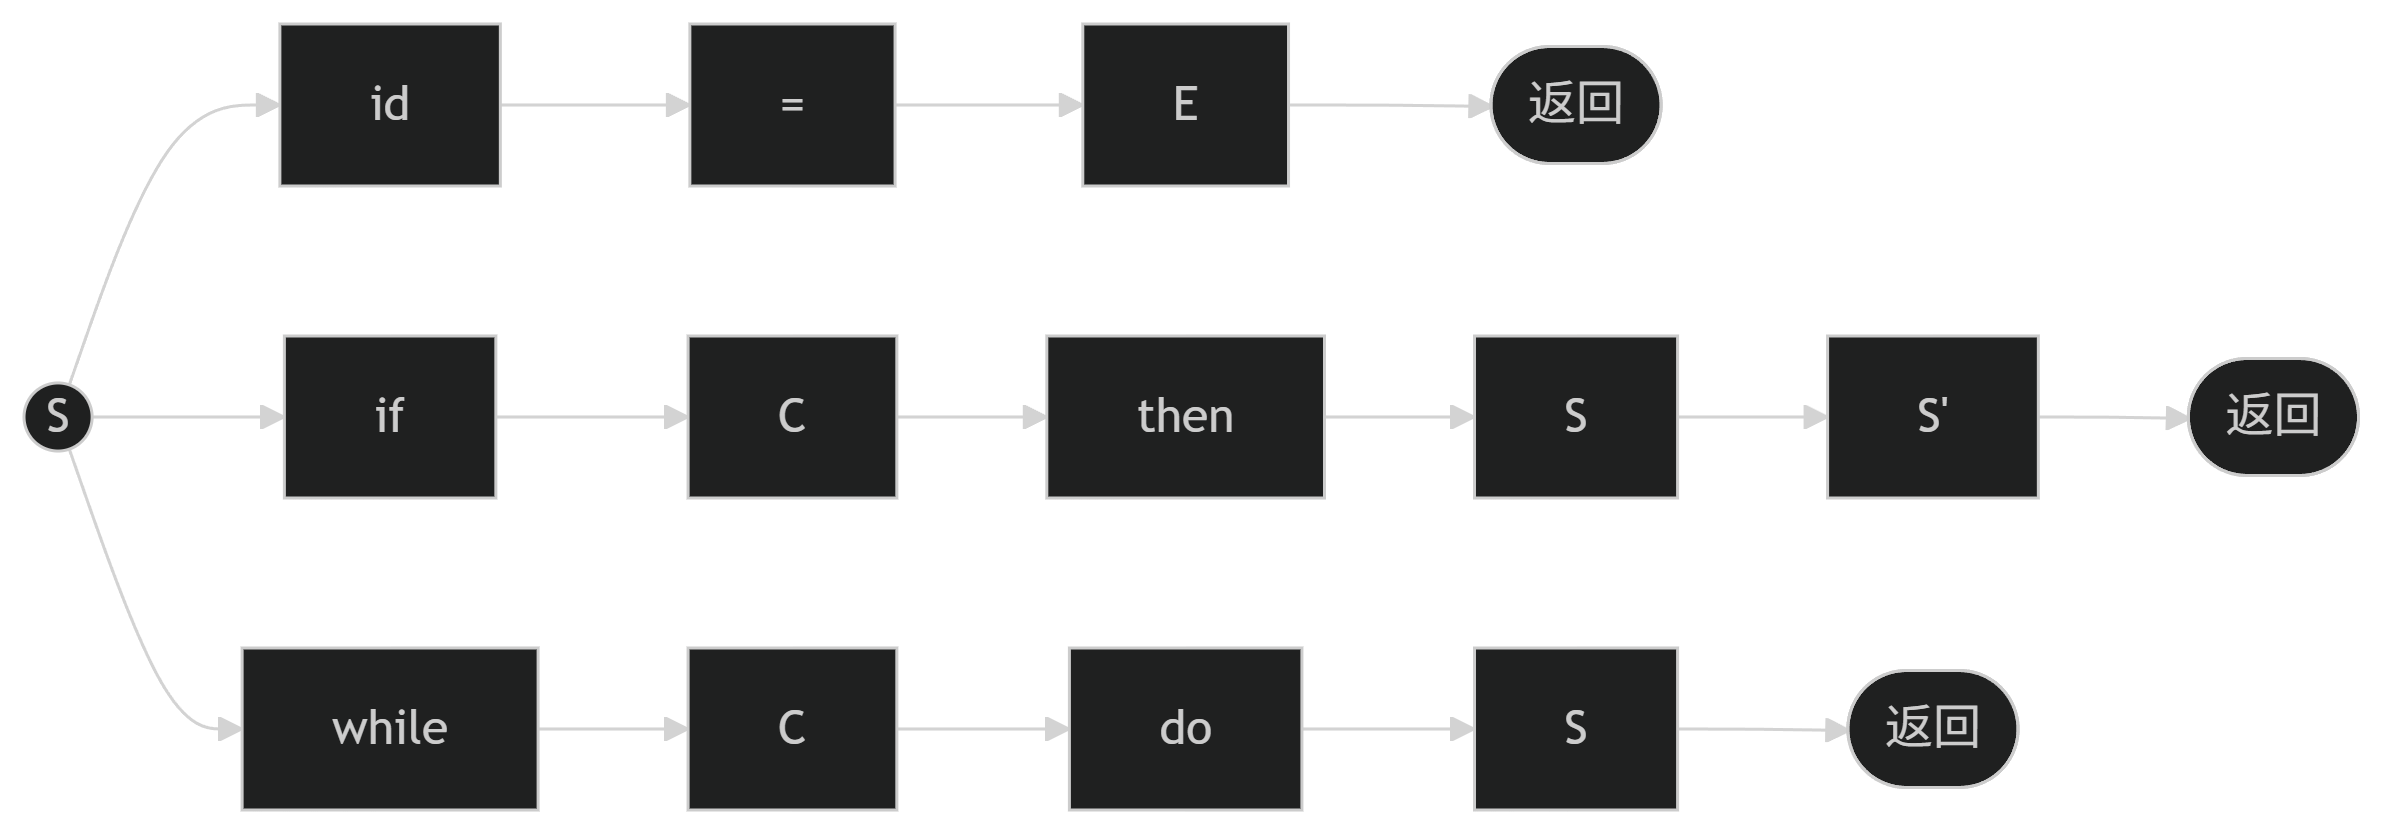
\includegraphics{member-sources/lab2-media/media/image1.png}
\caption{S 的语法图}
\end{figure}

\begin{figure}
\centering
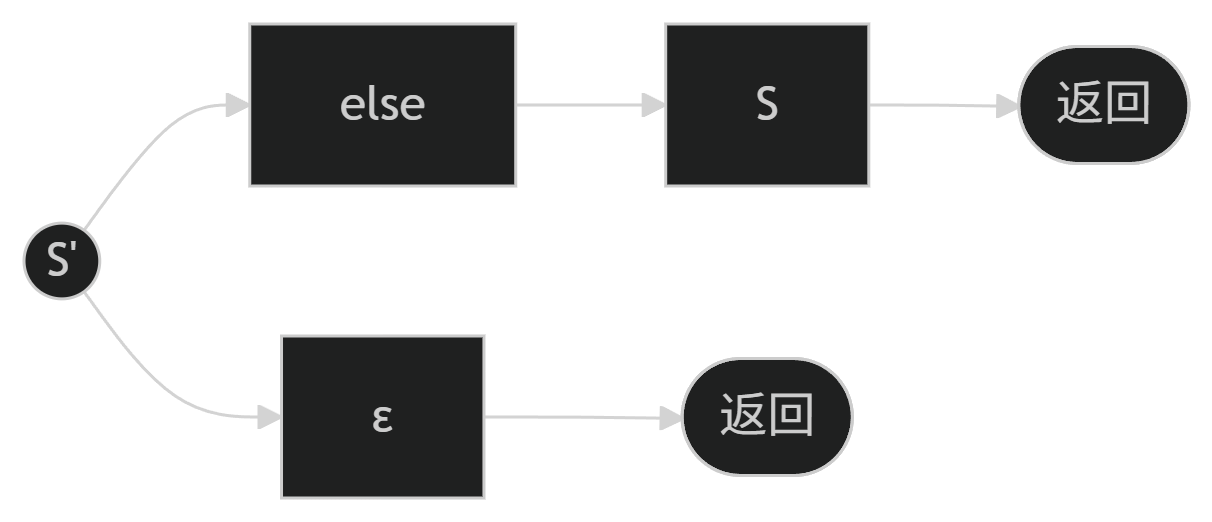
\includegraphics{member-sources/lab2-media/media/image2.png}
\caption{S' 的语法图}
\end{figure}

\begin{figure}
\centering
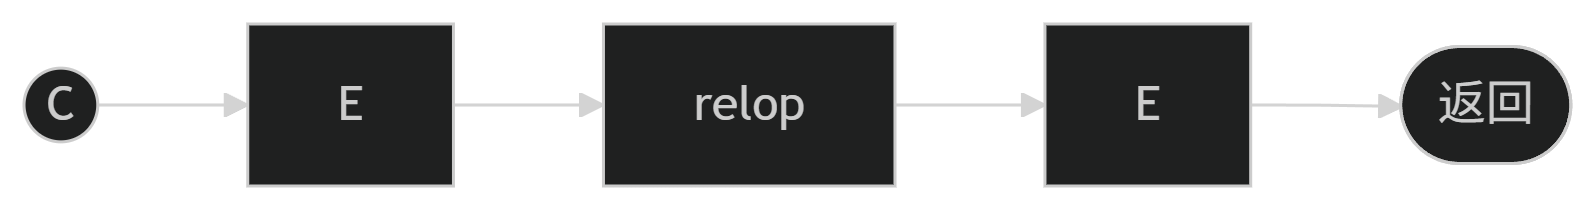
\includegraphics{member-sources/lab2-media/media/image3.png}
\caption{C 的语法图}
\end{figure}

\begin{figure}
\centering
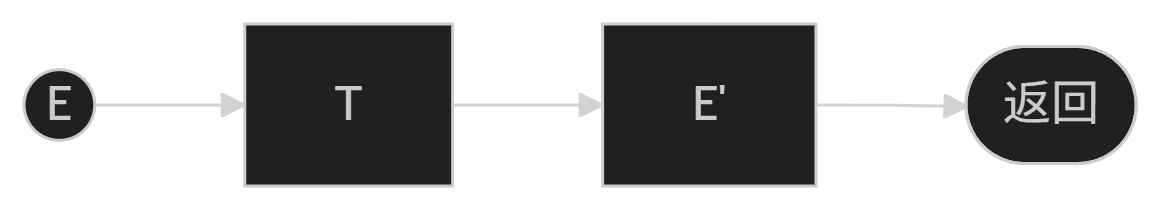
\includegraphics{member-sources/lab2-media/media/image4.png}
\caption{E 的语法图}
\end{figure}

\begin{figure}
\centering
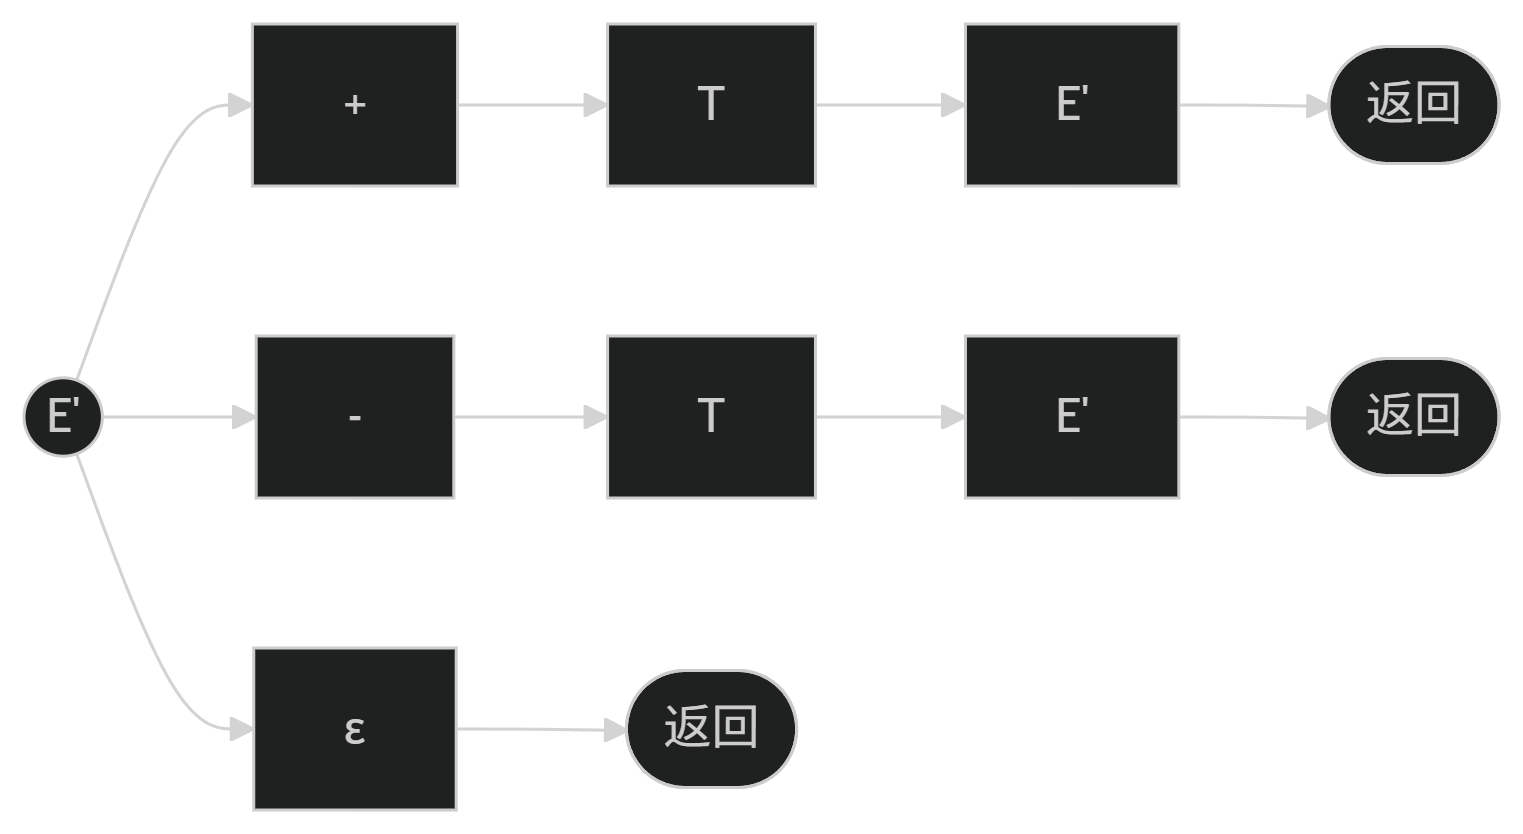
\includegraphics{member-sources/lab2-media/media/image5.png}
\caption{E' 的语法图}
\end{figure}

\begin{figure}
\centering
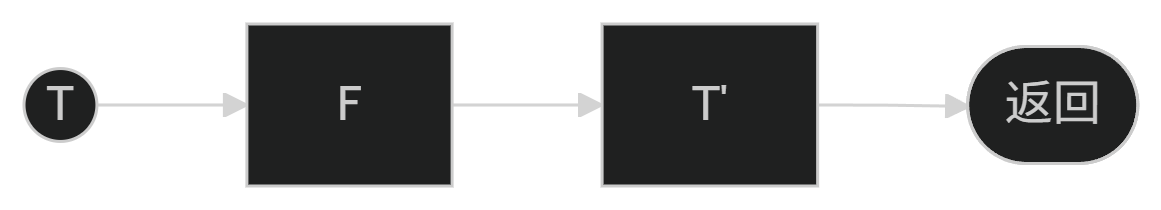
\includegraphics{member-sources/lab2-media/media/image6.png}
\caption{T 的语法图}
\end{figure}

\begin{figure}
\centering
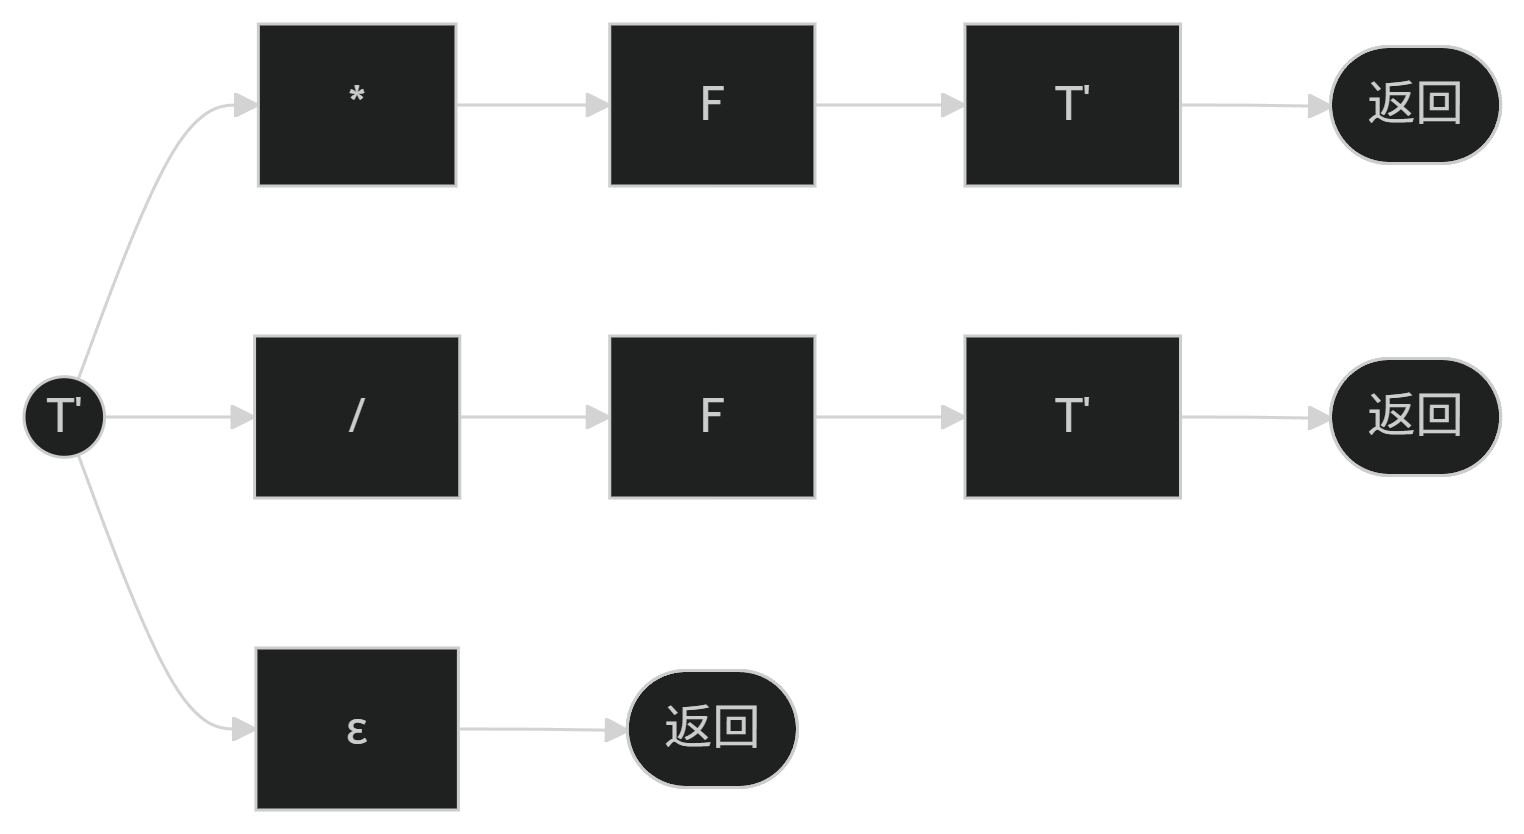
\includegraphics{member-sources/lab2-media/media/image7.png}
\caption{T' 的语法图}
\end{figure}

\begin{figure}
\centering
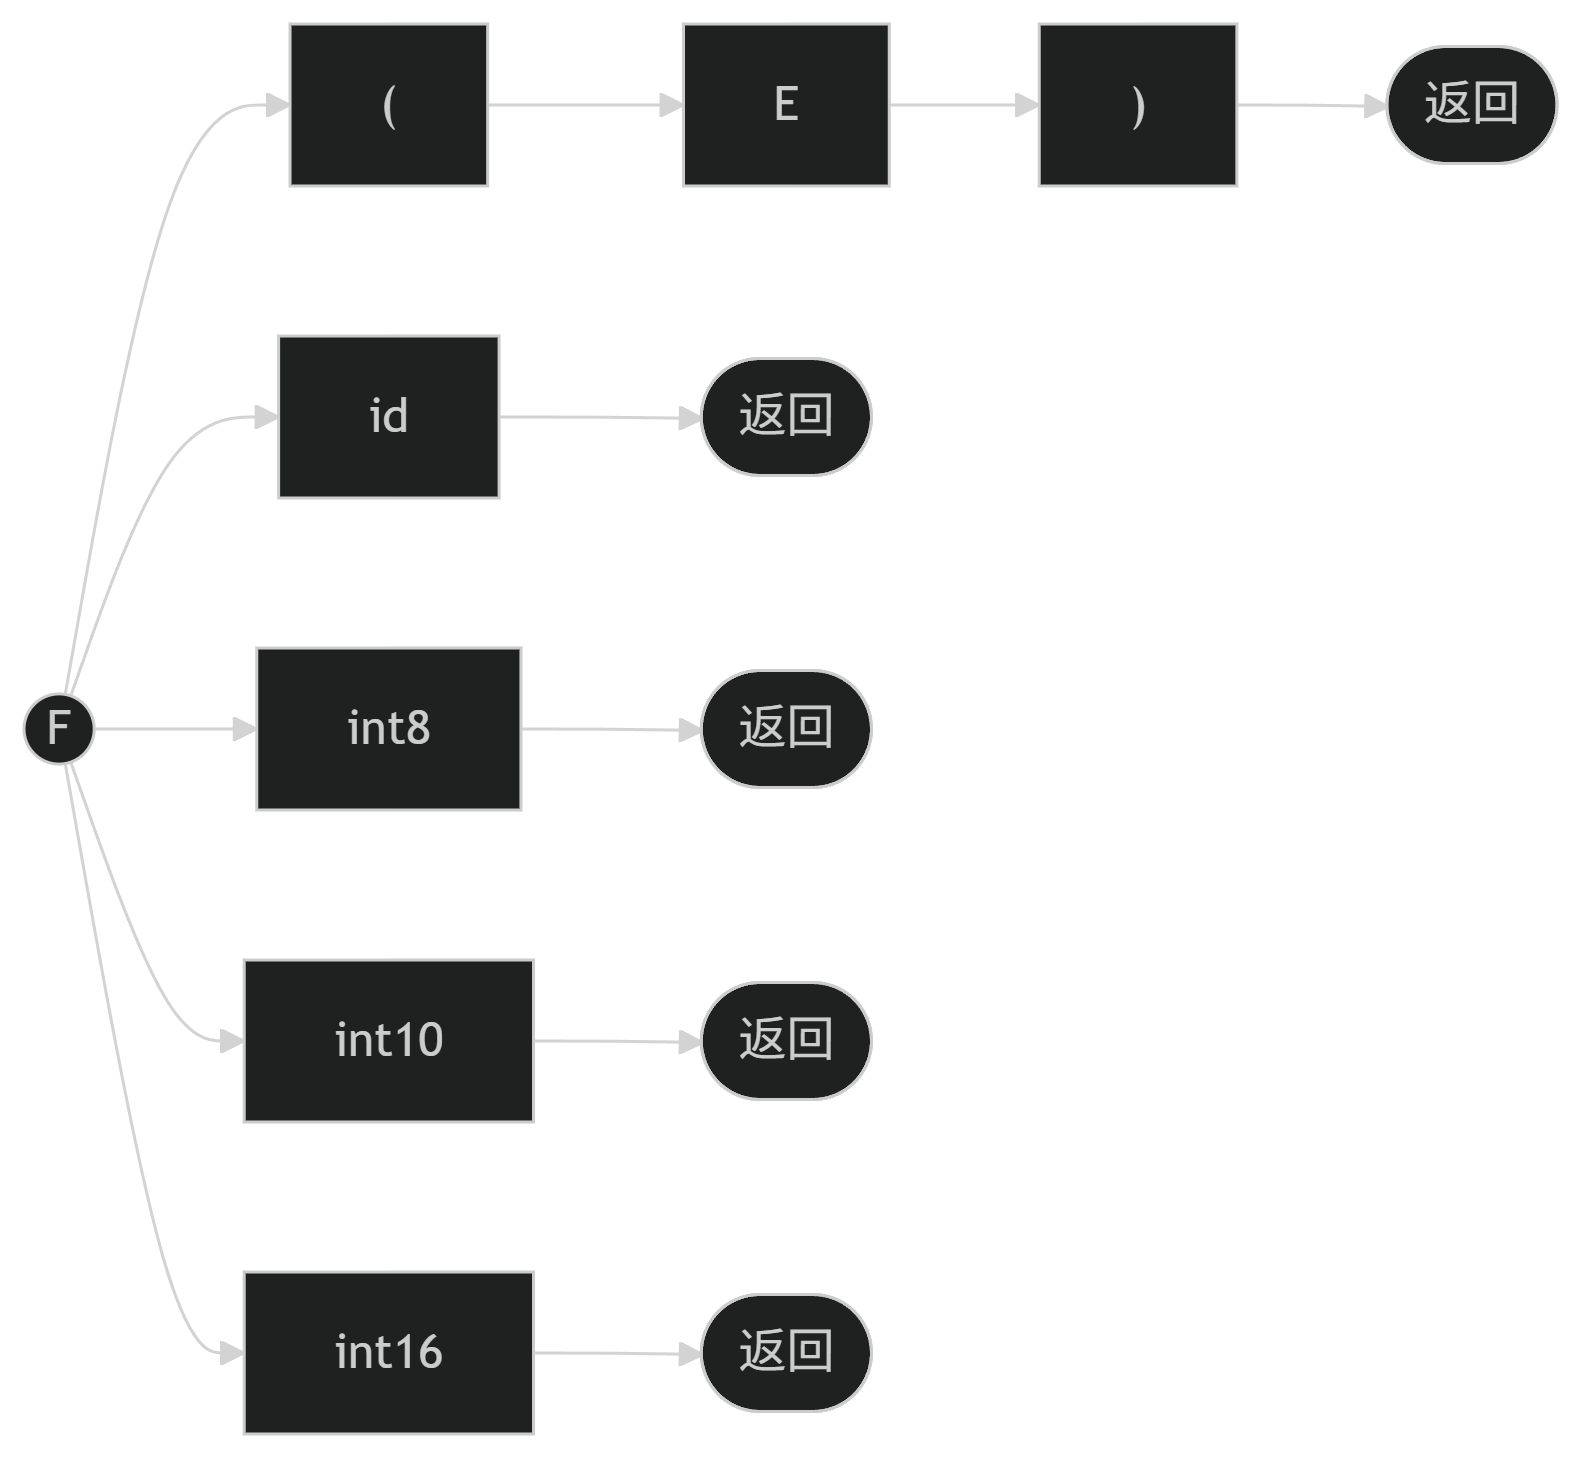
\includegraphics{member-sources/lab2-media/media/image8.png}
\caption{F 的语法图}
\end{figure}

\hypertarget{ux4e3bux8981ux6570ux636eux7ed3ux6784ux4e0eux51fdux6570-1}{%
\paragraph{5.1.3
主要数据结构与函数}\label{ux4e3bux8981ux6570ux636eux7ed3ux6784ux4e0eux51fdux6570-1}}

递归下降 parser 的主要状态：

\begin{Shaded}
\begin{Highlighting}[]
\NormalTok{lexer          : 共享词法器}
\NormalTok{lookahead      : 当前前看 token}
\NormalTok{indent         : 语法树输出缩进层级}
\NormalTok{errorCount     : 错误计数}
\NormalTok{errorMessages  : 错误信息列表}
\NormalTok{SYNC\_STMT      : 语句级同步集合}
\NormalTok{SYNC\_BLOCK     : 块级同步集合}
\end{Highlighting}
\end{Shaded}

主要函数：

\begin{longtable}[]{@{}ll@{}}
\toprule\noalign{}
函数 & 对应文法/职责 \\
\midrule\noalign{}
\endhead
\bottomrule\noalign{}
\endlastfoot
\texttt{parseProgram()} &
\texttt{P\ -\textgreater{}\ L+}，语法分析入口 \\
\texttt{parseL()} & \texttt{L\ -\textgreater{}\ S\ ;} \\
\texttt{parseS()} & 选择赋值、if、while、begin 分支 \\
\texttt{parseAssign()} & \texttt{S\ -\textgreater{}\ id\ =\ E} \\
\texttt{parseIf()} &
\texttt{S\ -\textgreater{}\ if\ C\ then\ S\ S\textquotesingle{}} \\
\texttt{parseWhile()} & \texttt{S\ -\textgreater{}\ while\ C\ do\ S} \\
\texttt{parseCompound()} &
\texttt{S\ -\textgreater{}\ begin\ L\_list\ end} \\
\texttt{parseLList()} & 复合语句内部语句列表 \\
\texttt{parseC()} & \texttt{C\ -\textgreater{}\ E\ relop\ E} \\
\texttt{parseRelop()} & 六种关系运算符 \\
\texttt{parseE()} &
\texttt{E\ -\textgreater{}\ T\ E\textquotesingle{}}，用循环处理加减 \\
\texttt{parseT()} &
\texttt{T\ -\textgreater{}\ F\ T\textquotesingle{}}，用循环处理乘除 \\
\texttt{parseF()} & 标识符、整数和括号表达式 \\
\texttt{match()} & 匹配终结符并推进 token \\
\texttt{error()} & 记录带行列号的错误信息 \\
\end{longtable}

\hypertarget{ux9012ux5f52ux4e0bux964dux7b97ux6cd5}{%
\paragraph{5.1.4
递归下降算法}\label{ux9012ux5f52ux4e0bux964dux7b97ux6cd5}}

算法流程：

\begin{Shaded}
\begin{Highlighting}[]
\NormalTok{1. 每个非终结符对应一个 parseXxx() 方法。}
\NormalTok{2. 方法内部通过 check(type) 判断 lookahead 的 token 类型。}
\NormalTok{3. 根据 FIRST 集选择产生式分支。}
\NormalTok{4. 遇到终结符时调用 match(type) 消费 token。}
\NormalTok{5. 遇到非终结符时递归调用对应 parseXxx() 方法。}
\NormalTok{6. E\textquotesingle{} 和 T\textquotesingle{} 使用 while 循环实现，避免直接左递归。}
\NormalTok{7. 出错时记录错误，并通过同步符号尝试继续分析。}
\end{Highlighting}
\end{Shaded}

\texttt{parseS()} 的分支选择：

\begin{Shaded}
\begin{Highlighting}[]
\NormalTok{if lookahead == IDN:}
\NormalTok{    S {-}\textgreater{} id = E}
\NormalTok{else if lookahead == IF:}
\NormalTok{    S {-}\textgreater{} if C then S S\textquotesingle{}}
\NormalTok{else if lookahead == WHILE:}
\NormalTok{    S {-}\textgreater{} while C do S}
\NormalTok{else if lookahead == BEGIN:}
\NormalTok{    S {-}\textgreater{} begin L\_list end}
\NormalTok{else:}
\NormalTok{    report error}
\end{Highlighting}
\end{Shaded}

\hypertarget{ux9012ux5f52ux4e0bux964dux6d4bux8bd5}{%
\paragraph{5.1.5
递归下降测试}\label{ux9012ux5f52ux4e0bux964dux6d4bux8bd5}}

运行命令：

\begin{Shaded}
\begin{Highlighting}[]
\ExtensionTok{java} \AttributeTok{{-}jar}\NormalTok{ dist/compiler{-}lab.jar tree }\OperatorTok{\textless{}}\NormalTok{ examples/lab2/tree{-}sample.in}
\end{Highlighting}
\end{Shaded}

语法树输出节选：

\begin{Shaded}
\begin{Highlighting}[]
\NormalTok{P    [P {-}\textgreater{} L+]}
\NormalTok{  L    [L {-}\textgreater{} S ;]}
\NormalTok{    S    [S {-}\textgreater{} while C do S]}
\NormalTok{      WHILE : while}
\NormalTok{      C    [C {-}\textgreater{} E relop E]}
\NormalTok{        E    [E {-}\textgreater{} T E\textquotesingle{}]}
\NormalTok{          T    [T {-}\textgreater{} F T\textquotesingle{}]}
\NormalTok{            F    [F {-}\textgreater{} ( E )]}
\NormalTok{              SLP : (}
\NormalTok{              E    [E {-}\textgreater{} T E\textquotesingle{}]}
\NormalTok{                T    [T {-}\textgreater{} F T\textquotesingle{}]}
\NormalTok{                  F    [F {-}\textgreater{} id]}
\NormalTok{                    IDN : a3}
\NormalTok{...}
\NormalTok{语法分析成功！}
\end{Highlighting}
\end{Shaded}

\hypertarget{ux9012ux5f52ux4e0bux964dux6269ux5c55}{%
\paragraph{5.1.6
递归下降扩展}\label{ux9012ux5f52ux4e0bux964dux6269ux5c55}}

递归下降语法分析支持以下扩展：

\begin{longtable}[]{@{}
  >{\raggedright\arraybackslash}p{(\columnwidth - 2\tabcolsep) * \real{0.5000}}
  >{\raggedright\arraybackslash}p{(\columnwidth - 2\tabcolsep) * \real{0.5000}}@{}}
\toprule\noalign{}
\begin{minipage}[b]{\linewidth}\raggedright
扩展
\end{minipage} & \begin{minipage}[b]{\linewidth}\raggedright
说明
\end{minipage} \\
\midrule\noalign{}
\endhead
\bottomrule\noalign{}
\endlastfoot
全部六种关系运算符 & \texttt{parseRelop()} 支持
\texttt{GT}、\texttt{LT}、\texttt{EQ}、\texttt{GE}、\texttt{LE}、\texttt{NEQ} \\
复合语句 & 新增 \texttt{S\ -\textgreater{}\ begin\ L\_list\ end} 与
\texttt{L\_list\ -\textgreater{}\ S\ ;\ L\_list\ \textbar{}\ S\ ;} \\
非法数值检测与定位 & 词法层识别 \texttt{ILOCT}、\texttt{ILHEX}，语法层
\texttt{parseF()} 检测 \\
进制自动转换 & \texttt{Lexer.convertBaseToDecimal(text,\ base)}
将八/十六进制转十进制属性值 \\
错误定位 & \texttt{Token.line}、\texttt{Token.column} 与
\texttt{Lexer.advancePos()} 维护行列 \\
续编译 & 出错后跳到同步符号继续分析，最终汇总错误 \\
\end{longtable}

Lab 2 扩展测试截图说明如下。

用例 1：缺少分号隐式纠错。 测试目标是验证 \texttt{begin...end}
内语句缺分号时的隐式分号纠正。输入为
\texttt{begin\ x\ =\ 1\ y\ =\ 2\ end}。预期行为是 \texttt{x=1}
后自动补分号，\texttt{y=2} 后自动补分号，并输出语法树和 2 条警告。

\begin{figure}
\centering

\includegraphics{member-sources/lab2-media/media/image14.png}
\caption{Lab 2 缺少分号隐式纠错测试截图}
\end{figure}

用例 2：缺表达式续编译。
测试目标是验证等号后缺表达式时不会因第一个错误而停止。输入为
\texttt{begin\ x\ =\ ;\ y\ =\ 2;\ end}。预期行为是 \texttt{x=;}
处报告因子错误并继续分析，\texttt{y=2;} 正常解析，最终汇总 1 条错误。

\begin{figure}
\centering

\includegraphics{member-sources/lab2-media/media/image15.png}
\caption{Lab 2 缺表达式续编译测试截图}
\end{figure}

用例 3：非法整数错误定位。
测试目标是验证非法八进制和非法十六进制的精确错误定位。输入为
\texttt{begin\ x\ =\ 09;\ y\ =\ 0xg;\ end}。预期行为是 \texttt{09}
报告非法八进制，\texttt{0xg} 报告非法十六进制，输出语法树并汇总 2
条带行列号的错误。

\begin{figure}
\centering

\includegraphics{member-sources/lab2-media/media/image16.png}
\caption{Lab 2 非法整数错误定位测试截图}
\end{figure}

用例 4：混合多种错误综合续编译。
测试目标是验证多种错误共存时的续编译和错误汇总能力。输入为
\texttt{begin\ a\ =\ 08\ +\ ;\ b\ =\ ;\ c\ =\ a\ *\ b;\ end}。预期行为是对非法八进制、缺表达式等错误分别报告，\texttt{c=a*b;}
继续正常解析，最终汇总 3 条错误。

\begin{figure}
\centering
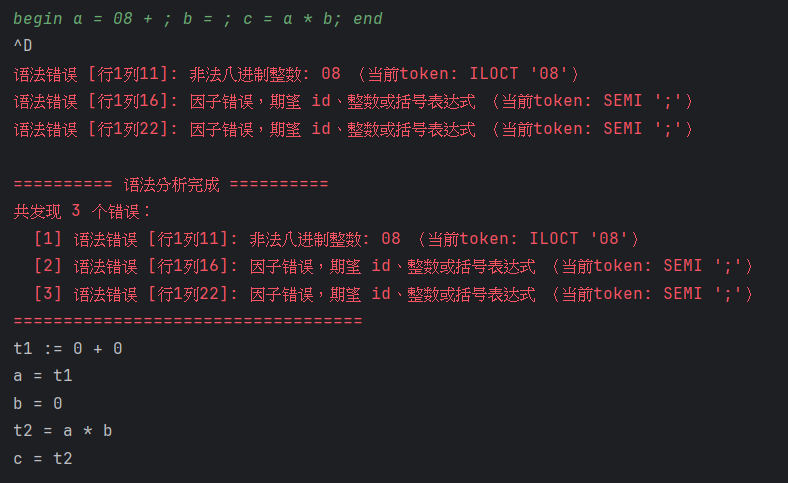
\includegraphics{member-sources/lab2-media/media/image17.png}
\caption{Lab 2 混合多种错误续编译测试截图}
\end{figure}

用例 5：六种关系符正常工作验证。 测试目标是验证全部六种关系运算符均被
\texttt{parseRelop()} 正确识别。输入包含 6 条 \texttt{if} 语句，分别使用
\texttt{\textgreater{}}、\texttt{\textless{}}、\texttt{=}、\texttt{\textgreater{}=}、\texttt{\textless{}=}、\texttt{\textless{}\textgreater{}}。预期行为是全部语句正常解析，语法树中依次出现六种关系运算符，无错误或警告。

\begin{figure}
\centering
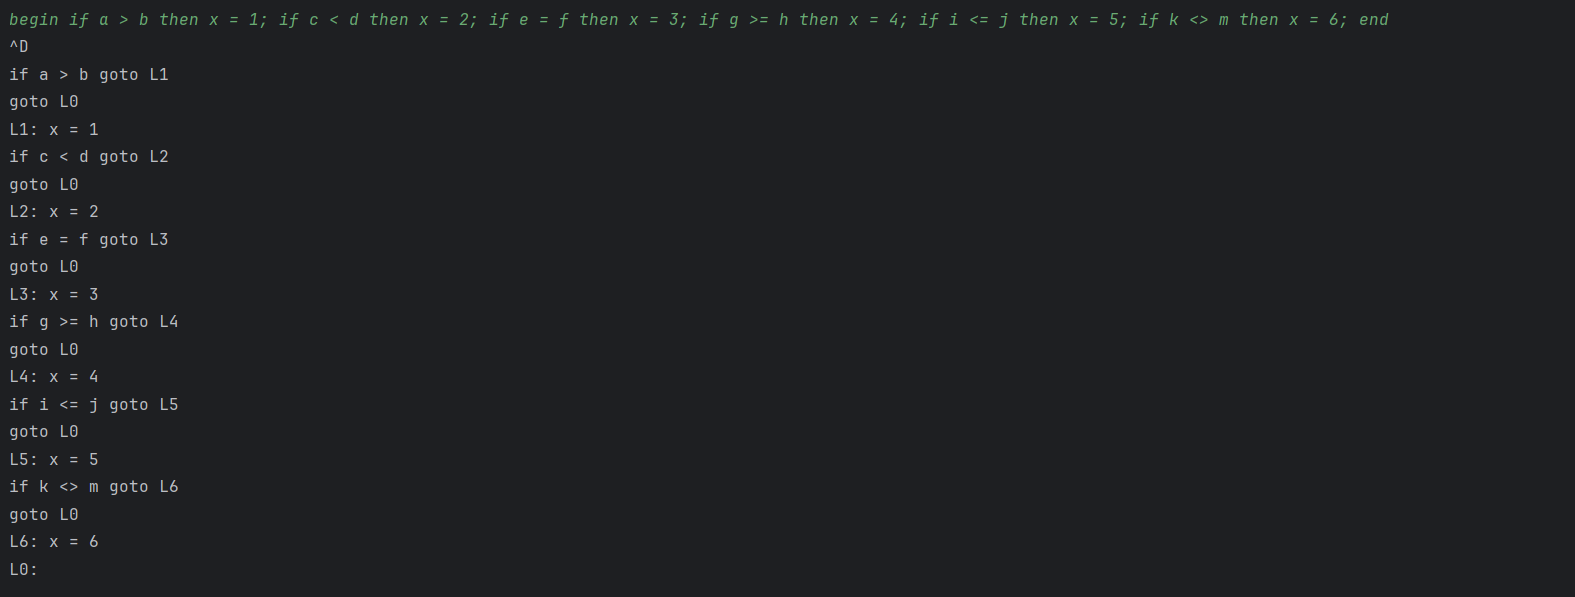
\includegraphics{member-sources/lab2-media/media/image18.png}
\caption{Lab 2 六种关系符验证测试截图}
\end{figure}

整合阶段补充了 \texttt{.in} 与 \texttt{.expected}
形式的自动化回归用例。非法八进制错误定位输出：

\begin{Shaded}
\begin{Highlighting}[]
\NormalTok{P    [P {-}\textgreater{} L+]}
\NormalTok{  L    [L {-}\textgreater{} S ;]}
\NormalTok{    S    [S {-}\textgreater{} id = E]}
\NormalTok{      IDN : x}
\NormalTok{      EQ : =}
\NormalTok{      E    [E {-}\textgreater{} T E\textquotesingle{}]}
\NormalTok{        T    [T {-}\textgreater{} F T\textquotesingle{}]}
\NormalTok{语法错误：非法八进制整数，当前单词为：ILOCT，属性值：{-}}
\end{Highlighting}
\end{Shaded}

关系运算符 token 验证输出节选：

\begin{Shaded}
\begin{Highlighting}[]
\NormalTok{GT {-}}
\NormalTok{LT {-}}
\NormalTok{EQ {-}}
\NormalTok{GE {-}}
\NormalTok{LE {-}}
\NormalTok{NEQ {-}}
\end{Highlighting}
\end{Shaded}

\hypertarget{ux81eaux5e95ux5411ux4e0abison-ux81eaux52a8ux751fux6210ux8bedux6cd5ux5206ux6790ux5668}{%
\subsubsection{5.2 自底向上：Bison
自动生成语法分析器}\label{ux81eaux5e95ux5411ux4e0abison-ux81eaux52a8ux751fux6210ux8bedux6cd5ux5206ux6790ux5668}}

\hypertarget{ux81eaux52a8ux751fux6210ux6280ux672f}{%
\paragraph{5.2.1
自动生成技术}\label{ux81eaux52a8ux751fux6210ux6280ux672f}}

实验三主语法分析路径使用 GNU Bison 生成 Java
parser。该部分属于自底向上的 LALR 分析器生成方法。

Bison 配置：

\begin{Shaded}
\begin{Highlighting}[]
\NormalTok{\%language "Java"}
\NormalTok{\%define api.parser.class \{TacBisonParser\}}
\NormalTok{\%define api.value.type \{Object\}}
\NormalTok{\%define parse.error verbose}
\end{Highlighting}
\end{Shaded}

描述程序：

\begin{Shaded}
\begin{Highlighting}[]
\NormalTok{src/TacBisonParser.y}
\end{Highlighting}
\end{Shaded}

生成程序：

\begin{Shaded}
\begin{Highlighting}[]
\NormalTok{build/generated/src/TacBisonParser.java}
\end{Highlighting}
\end{Shaded}

辅助程序：

\begin{longtable}[]{@{}ll@{}}
\toprule\noalign{}
文件 & 职责 \\
\midrule\noalign{}
\endhead
\bottomrule\noalign{}
\endlastfoot
\texttt{BisonTacParser.java} & 适配共享 \texttt{Lexer} 与 Bison parser
接口 \\
\texttt{TacAst.java} & 定义 Bison 规约动作构造的 AST 节点 \\
\texttt{TacAstPrinter.java} & 输出 AST 文本 \\
\texttt{TacAstDotPrinter.java} & 输出 AST 的 Graphviz DOT \\
\end{longtable}

\hypertarget{bison-ux6587ux6cd5}{%
\paragraph{5.2.2 Bison 文法}\label{bison-ux6587ux6cd5}}

核心文法：

\begin{Shaded}
\begin{Highlighting}[]
\NormalTok{program          {-}\textgreater{} top\_statements opt\_semi}
\NormalTok{top\_statements   {-}\textgreater{} statement}
\NormalTok{                  | top\_statements ; statement}
\NormalTok{opt\_semi         {-}\textgreater{} ε | ;}
\NormalTok{statement        {-}\textgreater{} id = expr}
\NormalTok{                  | if condition then statement}
\NormalTok{                  | if condition then statement else statement}
\NormalTok{                  | while condition do statement}
\NormalTok{                  | begin compound\_statements end}
\NormalTok{                  | error}
\NormalTok{compound\_stmt    {-}\textgreater{} statement ;}
\NormalTok{                  | compound\_stmt statement ;}
\NormalTok{condition        {-}\textgreater{} expr relop expr}
\NormalTok{relop            {-}\textgreater{} \textgreater{} | \textless{} | = | \textgreater{}= | \textless{}= | \textless{}\textgreater{}}
\NormalTok{expr             {-}\textgreater{} expr + expr}
\NormalTok{                  | expr {-} expr}
\NormalTok{                  | expr * expr}
\NormalTok{                  | expr / expr}
\NormalTok{                  | ( expr )}
\NormalTok{                  | factor}
\NormalTok{factor           {-}\textgreater{} id | int8 | int10 | int16}
\end{Highlighting}
\end{Shaded}

表达式优先级：

\begin{Shaded}
\begin{Highlighting}[]
\NormalTok{\%left ADD SUB}
\NormalTok{\%left MUL DIV}
\end{Highlighting}
\end{Shaded}

该声明等价于传统表达式文法中 \texttt{E/T/F}
的优先级分层。加减优先级低于乘除，括号通过 \texttt{SLP\ expr\ SRP}
改变归约结构。

dangling-else 处理：

\begin{Shaded}
\begin{Highlighting}[]
\NormalTok{\%nonassoc THEN}
\NormalTok{\%nonassoc ELSE}
\NormalTok{statement {-}\textgreater{} IF condition THEN statement \%prec THEN}
\NormalTok{statement {-}\textgreater{} IF condition THEN statement ELSE statement}
\end{Highlighting}
\end{Shaded}

该设计使 \texttt{else} 绑定到最邻近的未匹配 \texttt{if}。

\hypertarget{bison-parser-ux603bux4f53ux7ed3ux6784}{%
\paragraph{5.2.3 Bison parser
总体结构}\label{bison-parser-ux603bux4f53ux7ed3ux6784}}

Lab 3 的语法分析流程为：

\begin{Shaded}
\begin{Highlighting}[]
\NormalTok{Lexer}
\NormalTok{  {-}\textgreater{} BisonTacParser.TacLexerAdapter}
\NormalTok{  {-}\textgreater{} TacBisonParser}
\NormalTok{  {-}\textgreater{} TacProgram / TacStatement / TacExpr AST}
\end{Highlighting}
\end{Shaded}

\texttt{BisonTacParser.TacLexerAdapter} 的职责：

\begin{enumerate}
\def\labelenumi{\arabic{enumi}.}
\tightlist
\item
  调用共享 \texttt{Lexer.nextToken()}；
\item
  将 \texttt{Token.type} 映射为 Bison token 编号；
\item
  将 \texttt{Token} 作为 Bison 语义值传递给规约动作；
\item
  在 \texttt{yyerror()} 中记录带行列号的错误信息。
\end{enumerate}

\hypertarget{ast-ux6570ux636eux7ed3ux6784}{%
\paragraph{5.2.4 AST 数据结构}\label{ast-ux6570ux636eux7ed3ux6784}}

Bison 规约动作不直接生成三地址代码，而是构造 AST：

\begin{Shaded}
\begin{Highlighting}[]
\NormalTok{TacProgram  : List\textless{}TacStatement\textgreater{}}
\NormalTok{TacAssign   : id, expr}
\NormalTok{TacIf       : condition, thenBranch, elseBranch}
\NormalTok{TacWhile    : condition, body}
\NormalTok{TacCompound : List\textless{}TacStatement\textgreater{}}
\NormalTok{TacError    : 错误恢复产生的错误语句}

\NormalTok{TacValue       : 标识符或常量}
\NormalTok{TacBinary      : left, op, right}
\NormalTok{TacInvalidExpr : 非法 token 传播使用}

\NormalTok{TacCondition   : left, op, right}
\end{Highlighting}
\end{Shaded}

AST 文本输出：

\begin{Shaded}
\begin{Highlighting}[]
\NormalTok{Program}
\NormalTok{  While}
\NormalTok{    Condition \textless{}}
\NormalTok{      Value a}
\NormalTok{      Value b}
\NormalTok{    Compound}
\NormalTok{      Assign x}
\NormalTok{        Binary +}
\NormalTok{          Value x}
\NormalTok{          Value 1}
\NormalTok{      Assign y}
\NormalTok{        Binary *}
\NormalTok{          Value y}
\NormalTok{          Value 2}
\end{Highlighting}
\end{Shaded}

AST DOT 已由 Graphviz 渲染为下图。

\begin{figure}
\centering
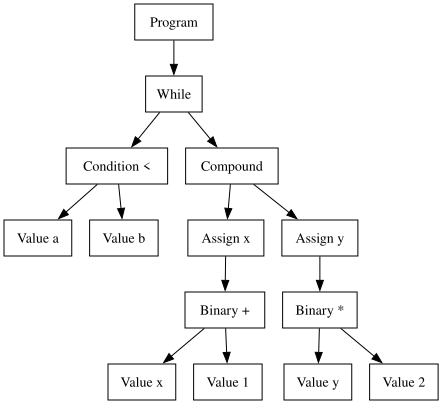
\includegraphics{assets/lab3-ast.pdf}
\caption{Bison AST 图}
\end{figure}

\hypertarget{ux9519ux8befux5904ux7406}{%
\paragraph{5.2.5 错误处理}\label{ux9519ux8befux5904ux7406}}

Bison 语法错误：

\begin{Shaded}
\begin{Highlighting}[]
\NormalTok{statement {-}\textgreater{} error}
\end{Highlighting}
\end{Shaded}

非法 token：

\begin{Shaded}
\begin{Highlighting}[]
\NormalTok{factor {-}\textgreater{} ILOCT}
\NormalTok{factor {-}\textgreater{} ILHEX}
\NormalTok{factor {-}\textgreater{} ILNUM}
\NormalTok{factor {-}\textgreater{} UNKNOWN}
\end{Highlighting}
\end{Shaded}

这些分支调用 \texttt{yyerror(...)}，然后返回
\texttt{TacInvalidExpr}。如果赋值表达式或条件表达式中包含
\texttt{TacInvalidExpr}，对应语句构造成 \texttt{TacError}。后续 TAC
生成阶段跳过 \texttt{TacError}，从而实现续编译。

错误恢复示例：

\begin{Shaded}
\begin{Highlighting}[]
\NormalTok{语法错误 [行1列5]: 非法八进制整数: 09（当前token: ILOCT \textquotesingle{}09\textquotesingle{}）}
\NormalTok{语法错误 [行2列5]: 非法十六进制整数: 0xg（当前token: ILHEX \textquotesingle{}0xg\textquotesingle{}）}
\NormalTok{语法错误 [行3列5]: 非法整数: 0abc（当前token: ILNUM \textquotesingle{}0abc\textquotesingle{}）}
\NormalTok{语法错误 [行4列5]: 无法识别的字符: \textquotesingle{}@\textquotesingle{}（当前token: UNKNOWN \textquotesingle{}@\textquotesingle{}）}
\NormalTok{ok = 1}
\end{Highlighting}
\end{Shaded}

\hypertarget{ux81eaux5e95ux5411ux4e0aux539fux7406ux5c55ux793aminiyaccslr}{%
\subsubsection{5.3
自底向上原理展示：MiniYacc/SLR}\label{ux81eaux5e95ux5411ux4e0aux539fux7406ux5c55ux793aminiyaccslr}}

\hypertarget{ux8bbeux8ba1ux5b9aux4f4d}{%
\paragraph{5.3.1 设计定位}\label{ux8bbeux8ba1ux5b9aux4f4d}}

实验指导书扩展项中提到``自己做一个 YACC''。本实现不以自制 YACC 替代 Lab
3 主线 Bison parser，而是提供固定表达式文法的 MiniYacc/SLR
原理展示，用于展示课上学习的 LR 分析表构造的关键步骤。

固定文法：

\begin{Shaded}
\begin{Highlighting}[]
\NormalTok{(0) S\textquotesingle{} {-}\textgreater{} E}
\NormalTok{(1) E {-}\textgreater{} E + T}
\NormalTok{(2) E {-}\textgreater{} T}
\NormalTok{(3) T {-}\textgreater{} T * F}
\NormalTok{(4) T {-}\textgreater{} F}
\NormalTok{(5) F {-}\textgreater{} ( E )}
\NormalTok{(6) F {-}\textgreater{} id}
\end{Highlighting}
\end{Shaded}

\hypertarget{ux4e3bux8981ux6570ux636eux7ed3ux6784ux4e0eux7b97ux6cd5}{%
\paragraph{5.3.2
主要数据结构与算法}\label{ux4e3bux8981ux6570ux636eux7ed3ux6784ux4e0eux7b97ux6cd5}}

\texttt{MiniSlrDemo} 的主要数据结构：

\begin{longtable}[]{@{}ll@{}}
\toprule\noalign{}
数据结构 & 含义 \\
\midrule\noalign{}
\endhead
\bottomrule\noalign{}
\endlastfoot
\texttt{Production} & 编号产生式，包含 \texttt{lhs} 和 \texttt{rhs} \\
\texttt{Item} & LR(0) 项，包含产生式和点位置 \\
\texttt{Automaton} & 项目集状态和 GOTO 转移 \\
\texttt{Transition} & 状态间带符号的转移 \\
\texttt{Table} & ACTION/GOTO 分析表 \\
\end{longtable}

核心算法：

\begin{Shaded}
\begin{Highlighting}[]
\NormalTok{1. 增广文法，加入 S\textquotesingle{} {-}\textgreater{} E。}
\NormalTok{2. 从 S\textquotesingle{} {-}\textgreater{} . E 出发计算 closure，得到 I0。}
\NormalTok{3. 对每个项目集和每个文法符号计算 goto(I, X)。}
\NormalTok{4. 如果 goto(I, X) 产生新项目集，则加入状态集合。}
\NormalTok{5. 重复直到没有新项目集。}
\NormalTok{6. 根据终结符转移填写 ACTION shift 项。}
\NormalTok{7. 根据完整项目和 FOLLOW 集填写 ACTION reduce 项。}
\NormalTok{8. 对 S\textquotesingle{} {-}\textgreater{} E . 填写 acc。}
\NormalTok{9. 根据非终结符转移填写 GOTO 表。}
\end{Highlighting}
\end{Shaded}

\hypertarget{ux5b9eux9a8cux8bc1ux636e}{%
\paragraph{5.3.3 实验证据}\label{ux5b9eux9a8cux8bc1ux636e}}

运行命令：

\begin{Shaded}
\begin{Highlighting}[]
\ExtensionTok{java} \AttributeTok{{-}jar}\NormalTok{ dist/compiler{-}lab.jar minislr}
\ExtensionTok{java} \AttributeTok{{-}jar}\NormalTok{ dist/compiler{-}lab.jar minislr{-}dot}
\end{Highlighting}
\end{Shaded}

ACTION/GOTO 表节选：

\begin{Shaded}
\begin{Highlighting}[]
\NormalTok{MiniYacc SLR(1) Demo}

\NormalTok{Grammar:}
\NormalTok{  (0) S\textquotesingle{} {-}\textgreater{} E}
\NormalTok{  (1) E {-}\textgreater{} E + T}
\NormalTok{  (2) E {-}\textgreater{} T}
\NormalTok{  (3) T {-}\textgreater{} T * F}
\NormalTok{  (4) T {-}\textgreater{} F}
\NormalTok{  (5) F {-}\textgreater{} ( E )}
\NormalTok{  (6) F {-}\textgreater{} id}

\NormalTok{Canonical LR(0) item sets:}
\NormalTok{I0:}
\NormalTok{  S\textquotesingle{} {-}\textgreater{} . E}
\NormalTok{  E {-}\textgreater{} . E + T}
\NormalTok{  E {-}\textgreater{} . T}
\NormalTok{  T {-}\textgreater{} . T * F}
\NormalTok{  T {-}\textgreater{} . F}
\NormalTok{  F {-}\textgreater{} . ( E )}
\NormalTok{  F {-}\textgreater{} . id}

\NormalTok{ACTION/GOTO table:}
\NormalTok{State | id | + | * | ( | ) | $ | E | T | F}
\NormalTok{0 | s5 |  |  | s4 |  |  | 1 | 2 | 3}
\NormalTok{1 |  | s6 |  |  |  | acc |  |  |}
\end{Highlighting}
\end{Shaded}

LR(0) 状态自动机 DOT 已渲染为下图。

\begin{figure}
\centering
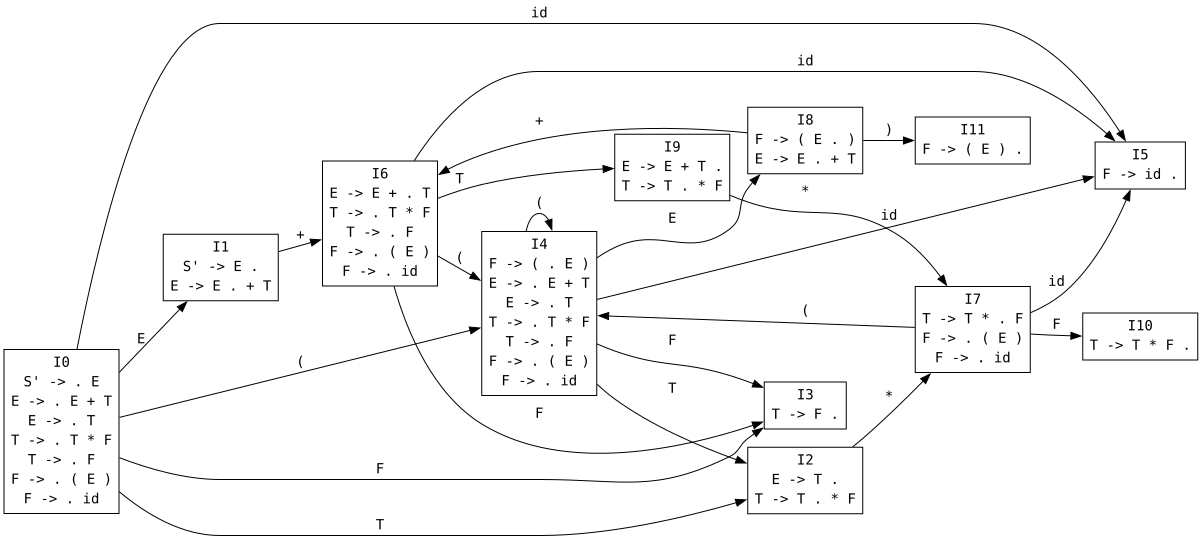
\includegraphics{assets/minislr-automaton.pdf}
\caption{MiniYacc SLR 自动机}
\end{figure}

\hypertarget{ux4e09ux5730ux5740ux4ee3ux7801ux751fux6210ux5668}{%
\subsection{6.
三地址代码生成器}\label{ux4e09ux5730ux5740ux4ee3ux7801ux751fux6210ux5668}}

\hypertarget{ux603bux4f53ux7ed3ux6784}{%
\subsubsection{6.1 总体结构}\label{ux603bux4f53ux7ed3ux6784}}

三地址代码生成器位于 Bison 语法分析之后：

\begin{Shaded}
\begin{Highlighting}[]
\NormalTok{TacProgram {-}\textgreater{} TacEmitter {-}\textgreater{} CodeGenerator {-}\textgreater{} TAC lines}
\end{Highlighting}
\end{Shaded}

Bison action 构造 AST，\texttt{TacEmitter} 遍历 AST
并按照实验指导书语法制导定义生成三地址代码，\texttt{CodeGenerator}
负责临时变量、标号和输出格式管理。

\hypertarget{ux8bedux6cd5ux5236ux5bfcux5b9aux4e49ux4e0eux5b9eux73b0}{%
\subsubsection{6.2
语法制导定义与实现}\label{ux8bedux6cd5ux5236ux5bfcux5b9aux4e49ux4e0eux5b9eux73b0}}

赋值语句：

\begin{Shaded}
\begin{Highlighting}[]
\NormalTok{S {-}\textgreater{} id = E}
\NormalTok{S.code = E.code || gen(id.place := E.place)}
\end{Highlighting}
\end{Shaded}

实现函数：

\begin{Shaded}
\begin{Highlighting}[]
\NormalTok{TacEmitter.emitAssign(TacAssign statement)}
\end{Highlighting}
\end{Shaded}

算法：

\begin{Shaded}
\begin{Highlighting}[]
\NormalTok{place = emitExpr(statement.expr)}
\NormalTok{emit(statement.id + " = " + place)}
\end{Highlighting}
\end{Shaded}

条件语句：

\begin{Shaded}
\begin{Highlighting}[]
\NormalTok{S {-}\textgreater{} if C then S1}
\NormalTok{C.true = newlabel}
\NormalTok{C.false = S.next}
\NormalTok{S.code = C.code || gen(C.true:) || S1.code}
\end{Highlighting}
\end{Shaded}

\texttt{if-else}：

\begin{Shaded}
\begin{Highlighting}[]
\NormalTok{S {-}\textgreater{} if C then S1 else S2}
\NormalTok{C.true = newlabel}
\NormalTok{C.false = newlabel}
\NormalTok{S1.next = S2.next = S.next}
\NormalTok{S.code = C.code || gen(C.true:) || S1.code}
\NormalTok{       || gen(goto S.next) || gen(C.false:) || S2.code}
\end{Highlighting}
\end{Shaded}

实现函数：

\begin{Shaded}
\begin{Highlighting}[]
\NormalTok{TacEmitter.emitIf(TacIf statement, String nextLabel)}
\end{Highlighting}
\end{Shaded}

循环语句：

\begin{Shaded}
\begin{Highlighting}[]
\NormalTok{S {-}\textgreater{} while C do S1}
\NormalTok{S.begin = newlabel}
\NormalTok{C.true = newlabel}
\NormalTok{C.false = S.next}
\NormalTok{S1.next = S.begin}
\NormalTok{S.code = gen(S.begin:) || C.code || gen(C.true:) || S1.code || gen(goto S.begin)}
\end{Highlighting}
\end{Shaded}

实现函数：

\begin{Shaded}
\begin{Highlighting}[]
\NormalTok{TacEmitter.emitWhile(TacWhile statement, String nextLabel, String currentLabel)}
\end{Highlighting}
\end{Shaded}

条件表达式：

\begin{Shaded}
\begin{Highlighting}[]
\NormalTok{C {-}\textgreater{} E1 relop E2}
\NormalTok{C.code = E1.code || E2.code}
\NormalTok{       || gen(if E1.place relop E2.place goto C.true)}
\NormalTok{       || gen(goto C.false)}
\end{Highlighting}
\end{Shaded}

实现函数：

\begin{Shaded}
\begin{Highlighting}[]
\NormalTok{TacEmitter.emitCondition(TacCondition condition, String trueLabel, String falseLabel)}
\end{Highlighting}
\end{Shaded}

算术表达式：

\begin{Shaded}
\begin{Highlighting}[]
\NormalTok{E {-}\textgreater{} E1 op T}
\NormalTok{E.place = newtemp}
\NormalTok{E.code = E1.code || T.code || gen(E.place := E1.place op T.place)}
\end{Highlighting}
\end{Shaded}

实现函数：

\begin{Shaded}
\begin{Highlighting}[]
\NormalTok{TacEmitter.emitExpr(TacExpr expr)}
\NormalTok{CodeGenerator.newTemp()}
\end{Highlighting}
\end{Shaded}

\hypertarget{codegenerator-ux6570ux636eux7ed3ux6784}{%
\subsubsection{6.3 CodeGenerator
数据结构}\label{codegenerator-ux6570ux636eux7ed3ux6784}}

\begin{longtable}[]{@{}ll@{}}
\toprule\noalign{}
字段/函数 & 作用 \\
\midrule\noalign{}
\endhead
\bottomrule\noalign{}
\endlastfoot
\texttt{tempCount} & 生成 \texttt{t1}、\texttt{t2}、\ldots{} \\
\texttt{labelCount} & 生成 \texttt{L1}、\texttt{L2}、\ldots{} \\
\texttt{usedProgramNextLabel} & 保证首个程序级汇合标签为 \texttt{L0} \\
\texttt{codes} & 保存 TAC 指令序列 \\
\texttt{referencedLabels} & 记录实际被跳转引用的标签 \\
\texttt{newTemp()} & 创建临时变量 \\
\texttt{newLabel()} & 创建普通标签 \\
\texttt{newProgramNextLabel()} & 创建程序级后继标签 \\
\texttt{emit()} & 输出普通 TAC \\
\texttt{emitLabel()} & 输出标签 \\
\texttt{emitGoto()} & 输出跳转并记录标签引用 \\
\texttt{patchGoto()} & 回填跳转目标 \\
\texttt{getCodes()} & 格式化输出，尽量将标签和下一条指令合并 \\
\end{longtable}

\hypertarget{ux6807ux51c6ux6837ux4f8bux8f93ux51fa}{%
\subsubsection{6.4
标准样例输出}\label{ux6807ux51c6ux6837ux4f8bux8f93ux51fa}}

运行命令：

\begin{Shaded}
\begin{Highlighting}[]
\ExtensionTok{java} \AttributeTok{{-}jar}\NormalTok{ dist/compiler{-}lab.jar tac }\OperatorTok{\textless{}}\NormalTok{ examples/lab3/handout{-}tac.in}
\end{Highlighting}
\end{Shaded}

输出：

\begin{Shaded}
\begin{Highlighting}[]
\NormalTok{L1: t1 := a3 + 15}
\NormalTok{if t1 \textgreater{} 10 goto L2}
\NormalTok{goto L0}
\NormalTok{L2: if x2 = 7 goto L3}
\NormalTok{goto L1}
\NormalTok{L3: if y \textless{} z goto L4}
\NormalTok{goto L1}
\NormalTok{L4: t2 = x * y}
\NormalTok{t3 = t2 / z}
\NormalTok{y = t3}
\NormalTok{goto L3}
\NormalTok{goto L1}
\NormalTok{L0: t4 = b * c}
\NormalTok{t5 = t4 + d}
\NormalTok{c = t5}
\end{Highlighting}
\end{Shaded}

\hypertarget{ux6269ux5c55ux5185ux5bb9}{%
\subsection{7. 扩展内容}\label{ux6269ux5c55ux5185ux5bb9}}

\hypertarget{ux5168ux90e8ux516dux79cdux5173ux7cfbux8fd0ux7b97ux7b26}{%
\subsubsection{7.1
全部六种关系运算符}\label{ux5168ux90e8ux516dux79cdux5173ux7cfbux8fd0ux7b97ux7b26}}

递归下降路径和 Bison 路径均支持：

\begin{Shaded}
\begin{Highlighting}[]
\NormalTok{relop {-}\textgreater{} \textgreater{} | \textless{} | = | \textgreater{}= | \textless{}= | \textless{}\textgreater{}}
\end{Highlighting}
\end{Shaded}

输出示例：

\begin{Shaded}
\begin{Highlighting}[]
\NormalTok{if a \textgreater{}= b goto L1}
\NormalTok{goto L0}
\NormalTok{L1: x = 1}
\NormalTok{L0: if a \textless{}= b goto L3}
\NormalTok{goto L2}
\NormalTok{L3: y = 2}
\NormalTok{L2: if a \textless{}\textgreater{} b goto L5}
\NormalTok{goto L4}
\NormalTok{L5: z = 3}
\NormalTok{L4:}
\end{Highlighting}
\end{Shaded}

\hypertarget{ux590dux5408ux8bedux53e5}{%
\subsubsection{7.2 复合语句}\label{ux590dux5408ux8bedux53e5}}

递归下降路径中：

\begin{Shaded}
\begin{Highlighting}[]
\NormalTok{S {-}\textgreater{} begin L\_list end}
\NormalTok{L\_list {-}\textgreater{} S ; L\_list | S ;}
\end{Highlighting}
\end{Shaded}

Bison 路径中：

\begin{Shaded}
\begin{Highlighting}[]
\NormalTok{statement {-}\textgreater{} BEGIN compound\_statements END}
\NormalTok{compound\_statements {-}\textgreater{} statement SEMI}
\NormalTok{                    | compound\_statements statement SEMI}
\end{Highlighting}
\end{Shaded}

输出示例：

\begin{Shaded}
\begin{Highlighting}[]
\NormalTok{L1: if a \textless{} b goto L2}
\NormalTok{goto L0}
\NormalTok{L2: t1 := x + 1}
\NormalTok{x = t1}
\NormalTok{t2 = y * 2}
\NormalTok{y = t2}
\NormalTok{goto L1}
\NormalTok{L0:}
\end{Highlighting}
\end{Shaded}

\hypertarget{ux9519ux8befux5b9aux4f4dux4e0eux7eedux7f16ux8bd1}{%
\subsubsection{7.3
错误定位与续编译}\label{ux9519ux8befux5b9aux4f4dux4e0eux7eedux7f16ux8bd1}}

非法 token 恢复输出：

\begin{Shaded}
\begin{Highlighting}[]
\NormalTok{语法错误 [行1列5]: 非法八进制整数: 09（当前token: ILOCT \textquotesingle{}09\textquotesingle{}）}
\NormalTok{语法错误 [行2列5]: 非法十六进制整数: 0xg（当前token: ILHEX \textquotesingle{}0xg\textquotesingle{}）}
\NormalTok{语法错误 [行3列5]: 非法整数: 0abc（当前token: ILNUM \textquotesingle{}0abc\textquotesingle{}）}
\NormalTok{语法错误 [行4列5]: 无法识别的字符: \textquotesingle{}@\textquotesingle{}（当前token: UNKNOWN \textquotesingle{}@\textquotesingle{}）}
\NormalTok{ok = 1}
\end{Highlighting}
\end{Shaded}

前四条语句有错误，不生成 TAC；最后一条合法语句继续输出，体现续编译能力。

\hypertarget{ast-ux5c55ux793a}{%
\subsubsection{7.4 AST 展示}\label{ast-ux5c55ux793a}}

\texttt{-\/-ast} 和 \texttt{-\/-ast-dot} 用于展示 Bison parser
的中间结果。DOT 图已在语法分析子系统中展示。

\hypertarget{ux5e38ux91cfux6298ux53e0}{%
\subsubsection{7.5 常量折叠}\label{ux5e38ux91cfux6298ux53e0}}

\texttt{TacOptimizer.foldConstants()} 在 AST 层递归遍历表达式。当
\texttt{TacBinary} 左右两侧都是整数常量时，调用
\texttt{foldValues(left,\ op,\ right)} 计算结果，并替换为
\texttt{TacValue}。除法遇到除数 0 时不折叠。

输出示例：

\begin{Shaded}
\begin{Highlighting}[]
\NormalTok{x = 14}
\NormalTok{y = 2}
\NormalTok{t1 := a + 2}
\NormalTok{z = t1}
\end{Highlighting}
\end{Shaded}

\hypertarget{ux81eaux52a8ux5316ux6d4bux8bd5ux4e0eux53efux6267ux884cux7a0bux5e8f}{%
\subsection{8.
自动化测试与可执行程序}\label{ux81eaux52a8ux5316ux6d4bux8bd5ux4e0eux53efux6267ux884cux7a0bux5e8f}}

\hypertarget{ux81eaux52a8ux5316ux56deux5f52ux6d4bux8bd5}{%
\subsubsection{8.1
自动化回归测试}\label{ux81eaux52a8ux5316ux56deux5f52ux6d4bux8bd5}}

测试命令：

\begin{Shaded}
\begin{Highlighting}[]
\FunctionTok{date} \KeywordTok{\&\&} \FunctionTok{make}\NormalTok{ test}
\end{Highlighting}
\end{Shaded}

成功截图如下。

\begin{figure}
\centering
\includegraphics{assets/make-test-success.png}
\caption{date \&\& make test 成功截图}
\end{figure}

自动化用例通过结果：

\begin{Shaded}
\begin{Highlighting}[]
\NormalTok{ok lab1\_sample}
\NormalTok{ok lexer\_contract}
\NormalTok{ok lab2\_tree\_sample}
\NormalTok{ok lab2\_tree\_invalid\_octal}
\NormalTok{ok lab3\_tac\_sample}
\NormalTok{ok lab3\_tac\_precedence}
\NormalTok{ok lab3\_tac\_nested\_control}
\NormalTok{ok lab3\_tac\_relop\_extended}
\NormalTok{ok lab3\_tac\_compound}
\NormalTok{ok lab3\_tac\_dangling\_else}
\NormalTok{ok lab3\_tac\_error\_recovery}
\NormalTok{ok lab3\_tac\_error\_missing\_rparen}
\NormalTok{ok lab3\_tac\_error\_missing\_then}
\NormalTok{ok lab3\_tac\_error\_compound\_recovery}
\NormalTok{ok lab3\_tac\_error\_multiple}
\NormalTok{ok lab3\_tac\_error\_invalid\_lexemes}
\NormalTok{ok lab3\_tac\_error\_invalid\_condition}
\NormalTok{ok lab3\_ast\_sample}
\NormalTok{ok lab3\_ast\_dot\_sample}
\NormalTok{ok lab3\_tac\_constant\_folding}
\NormalTok{ok minislr\_table}
\NormalTok{ok minislr\_dot}
\NormalTok{ok jar\_lab1\_sample}
\NormalTok{ok jar\_lab2\_tree\_sample}
\NormalTok{ok jar\_lab3\_tac\_sample}
\NormalTok{ok jar\_lab3\_tac\_constant\_folding}
\NormalTok{ok jar\_minislr\_table}
\end{Highlighting}
\end{Shaded}

测试覆盖：

\begin{itemize}
\tightlist
\item
  Lab 1 指导书样例；
\item
  共享 lexer 合同；
\item
  Lab 2 语法树输出和非法八进制错误；
\item
  Lab 3 指导书 TAC 样例；
\item
  表达式优先级、嵌套控制流；
\item
  扩展关系运算、复合语句、dangling else；
\item
  多类语法错误与非法 token 恢复；
\item
  AST 文本、AST DOT；
\item
  常量折叠；
\item
  MiniYacc/SLR 表和 DOT；
\item
  可执行 JAR 代表性 smoke tests。
\end{itemize}

\hypertarget{ux53efux6267ux884cux7a0bux5e8f}{%
\subsubsection{8.2 可执行程序}\label{ux53efux6267ux884cux7a0bux5e8f}}

构建：

\begin{Shaded}
\begin{Highlighting}[]
\FunctionTok{make}\NormalTok{ dist}
\end{Highlighting}
\end{Shaded}

生成：

\begin{Shaded}
\begin{Highlighting}[]
\NormalTok{dist/compiler{-}lab.jar}
\end{Highlighting}
\end{Shaded}

运行：

\begin{Shaded}
\begin{Highlighting}[]
\ExtensionTok{java} \AttributeTok{{-}jar}\NormalTok{ dist/compiler{-}lab.jar lab1 }\OperatorTok{\textless{}}\NormalTok{ examples/lab1/handout.in}
\ExtensionTok{java} \AttributeTok{{-}jar}\NormalTok{ dist/compiler{-}lab.jar tree }\OperatorTok{\textless{}}\NormalTok{ examples/lab2/tree{-}sample.in}
\ExtensionTok{java} \AttributeTok{{-}jar}\NormalTok{ dist/compiler{-}lab.jar tac }\OperatorTok{\textless{}}\NormalTok{ examples/lab3/handout{-}tac.in}
\ExtensionTok{java} \AttributeTok{{-}jar}\NormalTok{ dist/compiler{-}lab.jar tac{-}opt }\OperatorTok{\textless{}}\NormalTok{ examples/lab3/constant{-}folding.in}
\ExtensionTok{java} \AttributeTok{{-}jar}\NormalTok{ dist/compiler{-}lab.jar ast }\OperatorTok{\textless{}}\NormalTok{ examples/lab3/ast{-}sample.in}
\ExtensionTok{java} \AttributeTok{{-}jar}\NormalTok{ dist/compiler{-}lab.jar minislr}
\end{Highlighting}
\end{Shaded}

\hypertarget{ux5b9eux9a8cux4f53ux4f1a}{%
\subsection{9. 实验体会}\label{ux5b9eux9a8cux4f53ux4f1a}}

郑天白负责词法分析部分。在实现过程中，正规式、正规文法和状态图之间的对应关系更加清晰：正规式用于描述
token
集合，正规文法可以转换为状态机，而程序中的扫描逻辑实际上就是状态机的手工实现。非法八进制和非法十六进制的处理也说明，词法分析不仅要识别合法
token，还要尽可能保留非法词素，便于后续错误报告。

段晰迈负责递归下降语法分析部分。通过消除左递归、化简语法图、编写递归子程序，可以直观理解自顶向下语法分析的工作方式。\texttt{E\textquotesingle{}}
和 \texttt{T\textquotesingle{}}
的处理说明，文法变换不仅是理论步骤，也会直接影响程序结构。扩展关系运算符、复合语句和续编译能力时，需要同时考虑词法
token、语法产生式和错误同步点。

高子涵负责 Bison 路径和三地址代码生成部分。Bison 自动生成 parser
适合处理表达式优先级、dangling else 和错误恢复等语法问题；AST
中间表示使语法分析和语法制导翻译解耦，便于输出 AST、生成 TAC
和做常量折叠。MiniYacc/SLR 展示则帮助理解自动生成工具背后的 LR
项目集、GOTO 转移和 ACTION/GOTO 表构造过程。

全组联调过程中，测试用例和可执行程序非常重要。\texttt{make\ test}
将基本样例、扩展语法、错误恢复和可执行 JAR
都纳入验证，能够避免报告中的结论停留在文字描述层面。

\end{document}
